\documentclass{article}
\usepackage{graphicx}
\DeclareGraphicsExtensions{.pdf}

\usepackage[final]{pdfpages}

\headheight 0in
\oddsidemargin 0in
\evensidemargin  0in
\topmargin  -.25in
\textwidth 6.5in
\textheight 9in
\title{OMPT: An OpenMP\textsuperscript{\textregistered} Tools Application Programming Interface for Performance Analysis}
\author{Alexandre Eichenberger\thanks{IBM T.J. Watson Research Center}, 
John Mellor-Crummey\thanks{Rice University}, 
Martin Schulz\thanks{Lawrence Livermore National Laboratory},
\\~\\
Nawal Copty\thanks{Oracle}, 
Jim Cownie\thanks{Intel},
Tim Cramer\thanks{RWTH Aachen University}, 
% John DelSignore\thanks{Rogue Wave}, 
Robert Dietrich\thanks{TU Dresden, ZIH},
Xu Liu\hbox to 0in{$^\dagger$\hss},
Eugene Loh\hbox to 0in{$^\S$\hss}, 
Daniel Lorenz\thanks{J\"{u}lich Supercomputer Center}, 
\\
and other members of the OpenMP Tools Working Group}
\date{Revised November 6, 2015}

\usepackage{comment}
\usepackage{needspace}
\usepackage[colorlinks=true,citecolor=blue]{hyper ref}
\usepackage{url}
\usepackage{xcolor}

\newcommand{\descheader}[1]{{\needspace{3\baselineskip}\vspace{1em}\noindent \fbox{#1}}}


\begin{document}  
\begin{comment}   
\pagestyle{empty}
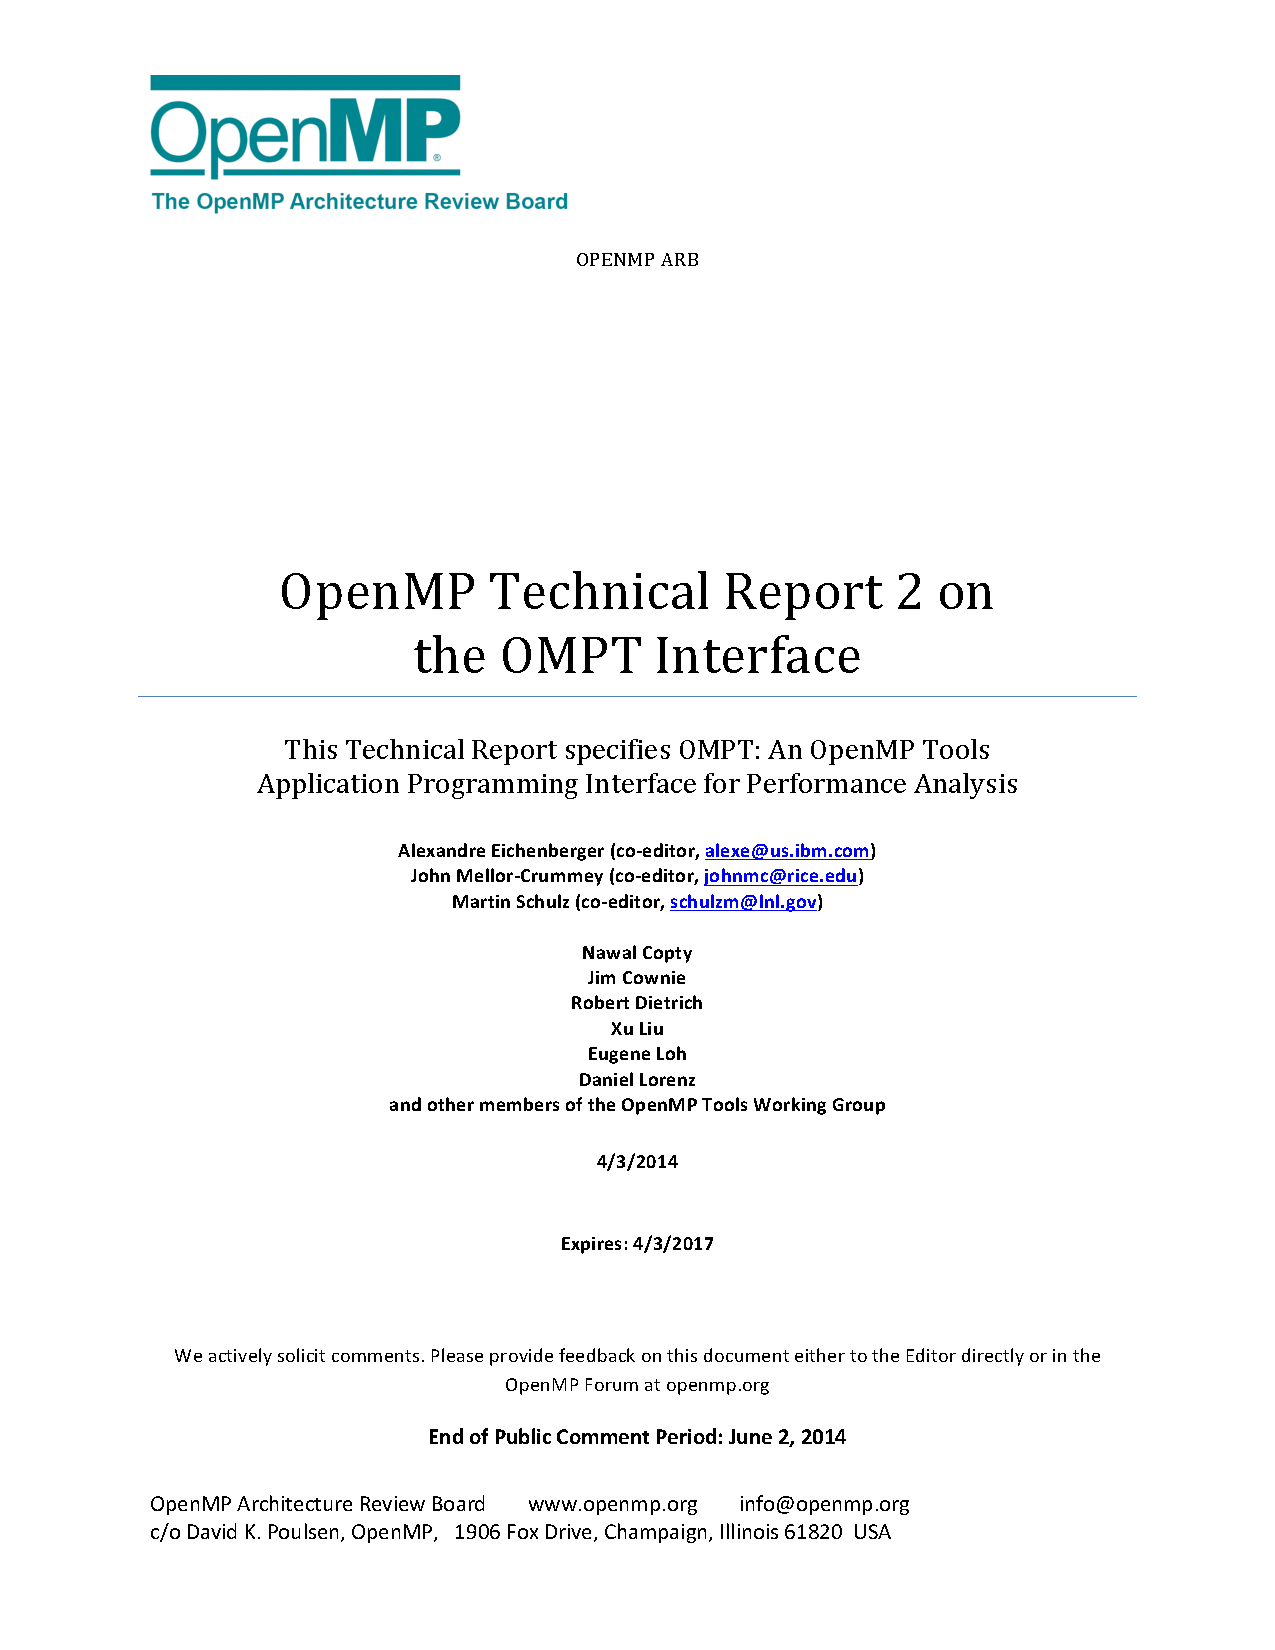
\includepdf[
   pages={-},
   pagecommand={},
 ]{OMPT_TR_header}
 
\setcounter{page}{1}
\pagestyle{plain}
\end{comment}
                                           
\maketitle
\section{Introduction}
Today, it is difficult to produce high quality tools that support 
% debugging and/or 
performance analysis of OpenMP programs without tightly integrating them with a specific OpenMP runtime implementation. To address this problem, this document defines OMPT---an application programming interface (API) for first-party performance tools.\footnote{A {\em first-party} tool runs within the address space of an application process. This differs from a {\em third-party} tool, e.g., a debugger, which runs as a separate process.}  
Extending the OpenMP standard with this API  will make it possible to construct powerful tools that will support any standard-compliant OpenMP implementation.


\begin{comment}
In appendices, we
define OMPD---an optional shared-library plugin that will enable debuggers  to inspect and control executions of OpenMP programs. We describe OMPD in this document because it provides third-party variants  of OMPT features  to enable assembly of user-level views of thread call stacks by debuggers.
\end{comment}

\subsection{OMPT}

The design of OMPT is based on experience with two prior efforts to define a standard OpenMP tools API: the POMP API~\cite{Mohr:EWOMP02} and the Sun/Oracle Collector API~\cite{SunCollector,Jost:2005:AND:1892830.1892858}. 
The POMP API provides support for instrumentation-based measurement. A drawback of this approach  is that its overhead can be significant because an operation, e.g., an iteration of an OpenMP worksharing loop, may take less time than tool callbacks monitoring its execution. 
%Doesn't have to be:
%Second, traces grow quickly and can be unwieldy for long executions. 
In contrast, 
the Sun/Oracle Collector API was  designed primarily to support performance measurement 
% and attribution of performance information 
using asynchronous sampling. This  design enables the construction of tools that attribute costs without the overhead and intrusion of pervasive instrumentation. With the Collector API, tools
 can use low-overhead asynchronous  sampling of application call stacks to record compact call path profiles. However, the Collector API doesn't provide enough instrumentation hooks to provide full tool support for statically-linked executables.
% instrumentation hooks to enable construction of trace analyzers or verification tools.
OMPT builds upon ideas from both the POMP and  Collector APIs. The core of OMPT is a minimal set of features to support tools that employ asynchronous sampling to measure application performance. In addition, OMPT defines  interfaces to support  {\em blame shifting}~\cite{Tallent:PPoPP09,Tallent:PPoPP10}---a technique that shifts attribution of costs from symptoms to causes.
Finally, OMPT defines callbacks suitable for instrumentation-based monitoring of runtime events. 
 OMPT can be implemented entirely by a compiler, entirely by an OpenMP runtime system, or with a hybrid strategy that employs a mixture of compiler and runtime support.
%equires no compiler support, and is implemented entirely within an OpenMP runtime system. 

With the exception of one routine for tool control, all functions in the OMPT API are intended for use only by tools rather than by applications. All OMPT API functions  have a C binding. A Fortran binding is  provided only for the single application-facing tool control function described in Section~\ref{sec:app-facing}.

\subsubsection{Design Objectives}
OMPT tries to satisfy several design objectives for a performance tool interface for OpenMP. These objectives are listed in decreasing order of importance.
\begin{itemize}
\item The  API should enable tools to gather sufficient information about an OpenMP program execution  to associate costs with both the program and the OpenMP runtime system.
\begin{itemize}
\item The  API should provide an interface sufficient to construct low-overhead performance tools based on asynchronous sampling.
\item The API should enable a profiler that uses call stack unwinding to identify which frames in its call stack are present on behalf of the OpenMP runtime.
\item An OpenMP runtime system should associate the activity of a thread at any point in time with a {\em state}, e.g., idle, which will enable a performance tool to interpret program behavior.  
\item Certain API routines must be defined as {\em async signal safe} so that they can be invoked in a profiler's signal handler as it processes interrupts generated by asynchronous sampling.
\end{itemize}
\item Incorporating support for the  API in an OpenMP runtime system should add negligible overhead to the runtime system if the interface is not in use by a tool.
\item The API should define interfaces suitable for constructing  instrumentation-based performance tools.
\item Adding the API to an OpenMP runtime should not impose an unreasonable development burden on the runtime developer.
\item The API should not impose an unreasonable development burden on tool implementers.
\end{itemize}

To support the OMPT interface for tools, an OpenMP runtime system must maintain information about the state of each OpenMP thread and provide a set of API calls that tools can use to interrogate the OpenMP runtime. Maintaining information about the state of each thread in the runtime system is not free and thus an OpenMP runtime system need not maintain state information unless a tool has registered its interest in this information.
% , or an environment variable has directed the tool to track runtime state.
Without any explicit request to enable tool support, an OpenMP runtime need not maintain any state for the benefit of tools.

\subsubsection{Minimally Compliant Implementation}

OMPT has a small set of mandatory features that provide a common foundation for all performance tools. A runtime may also implement additional, optional, OMPT features used by some tools to gather extra information about a program execution.     
The features required by a minimally compliant implementation are summarized below.

\begin{itemize}
\item Maintain a unique numerical ID per OpenMP thread, parallel region, and task region. A minimal implementation may reuse the task ID required by OpenMP for nested locks.
\item Maintain pointers into the stack for each OpenMP thread to distinguish frames for user procedures from frames for OpenMP runtime routines.  Each  OpenMP worker must maintain a pointer to the stack frame of the runtime routine containing its idle loop, if one exists on the stack. 
\item Maintain a state and a wait condition for each OpenMP thread. Mandatory states are idle, work serial, work parallel, and undefined.
\item Provide callbacks to tools when encountering the following  events:  thread begin/end, parallel region begin/end, task region begin/end, a user-level tool control call, and runtime shutdown.
\item Implement several async signal safe inquiry functions to retrieve information from the OpenMP runtime.
\item Have the OpenMP runtime initiate a callback to a tool initialization routine 
as directed by the value of a new OpenMP environment variable (\verb|OMP_TOOL|) and provide a function to register tool callbacks with the runtime.
\end{itemize}

\subsection{Document Roadmap}
This document first outlines various aspects of the OMPT tools API. 
Section~\ref{sec:states} describes the state information maintained by the OpenMP runtime system on behalf of OMPT for use by tools.
Section~\ref{sec:events} describes the OMPT callbacks to notify a tool of various OpenMP runtime events during an execution.
Section~\ref{sec:data} describes the data structures used by the OMPT interface.
Section~\ref{sec:inquiry} describes the runtime system inquiry operations supported by OMPT for the benefit of tools.
Section~\ref{sec:enabling} describes the OMPT API operations for tool initialization.
% Section~\ref{sec:globals} describes a global variable provided by the OpenMP runtime to support the OMPD debugger plug in library, which is being developed separately.
Section~\ref{sec:app-facing} describes the tool control interface available to applications.
Section~\ref{sec:notes} concludes with a few notes about potential future enhancements.
Appendix~\ref{appendix:ompt-types} provides a definition of the complete OMPT interface in C.
Appendix~\ref{app:frame} illustrates the information that OMPT maintains about call stacks and the use of OMPT API routines to inspect it; this support enables tools to associate code executed in OpenMP parallel regions with  application-level calling contexts. 
Appendix~\ref{app:registration} outlines some considerations that impact the design of the interface for tool registration.


\begin{comment}
Next, a pair of appendices describe OMPD---a shared library plugin for debuggers that supports third-party inspection and control of a target process. OMPD enables a debugger to leverage functionality provided by OMPT to enable it to provide a user-level view of call stacks for threads.
Appendix~\ref{appendix:ompd} describes the OMPD interface.  
Appendix~\ref{appendix:ompd-types} provides a definition of the complete OMPD interface in C.
\end{comment}

\section{Runtime States} 
\label{sec:states} 

To enable a tool to understand what an OpenMP thread is doing, when a tool registers itself with an OpenMP runtime system, the runtime 
will maintain state information for each OpenMP thread that can be queried by the tool. 
The state maintained for each thread by the OpenMP runtime is an
approximation of the thread's instantaneous state. 
OMPT uses the enumeration type \verb|ompt_state_t| for states;
Appendix~\ref{appendix:ompt-types:states} defines this type.
When the state of a thread not associated with the OpenMP runtime is queried, the runtime returns 
\verb|ompt_state_undefined|.

For each OpenMP thread the runtime maintains not only a state but also an \verb|ompt_wait_id_t|
identifier.  When a thread is waiting for a lock, critical region,
ordered, or atomic, and the thread is in a wait
state, then 
the thread's \verb|wait_id| field identifies the lock, critical construct, ordered construct, atomic construct, or internal variable
upon which the
thread is waiting. The semantics of the values used for a \verb|wait_id| are implementation defined.
A thread's \verb|wait_id| is undefined if the thread
is not in a wait state.

% States are classified as {\em mandatory} or {\em optional}.
Some states must be supported by any compliant implementation, e.g., those indicating that a thread is executing parallel or serial work. In other cases, alternatives exist. For instance, one may use a single state to represent all waiting at barriers or use a pair of states to differentiate between waiting at implicit and explicit barriers.
For some states, OpenMP runtimes have some flexibility about whether to report the state early or late.
For example, consider when a thread acquires a lock. One
compliant runtime may transition a thread's state to 
\verb|ompt_state_wait_lock|  early before the thread attempts to acquire a
lock. Another compliant runtime may transition a thread's state to
\verb|ompt_state_wait_lock| late, only if the thread begins to spin or
block to wait for an unavailable lock. A third compliant runtime
may transition a thread's state to \verb|ompt_state_wait_lock| even later, e.g., only
after the thread waits for a significant amount of time. 
% While flexible states are not mandatory as ``significant amount of time" is  not precisely defined, implementing them is recommended.

State values 0 to 127 are reserved for current OMPT states and future extensions.  

\descheader{Idle State}

\begin{description}
\item \verb|ompt_state_idle| 

  The thread is idle, waiting for work.
\end{description}

\descheader{Work States}

\begin{description}

\item \verb|ompt_state_work_serial| 

  The thread is executing code outside all parallel regions. 

\item \verb|ompt_state_work_parallel| 

  The thread is executing code within the scope of a parallel region construct.

\sloppy
\item \verb|ompt_state_work_reduction| 
 
  The thread is combining partial reduction results from threads in its team. A compliant
  runtime might never report a thread in this state; a thread
  combining partial reduction results may  report its state as
  \verb|ompt_state_work_parallel| or \verb|ompt_state_overhead|.

\end{description}

\descheader{Barrier Wait States}

\begin{description}

  \item \verb|ompt_state_wait_barrier| 
  
  \sloppy
  The thread is waiting at either an implicit or explicit barrier.
  A  compliant implementation may have a thread enter this state
  early, when the thread encounters a barrier, or late, when the
  thread begins to wait at the barrier. A  compliant implementation may never report a thread in this state; instead, a thread might report its state as \verb|ompt_state_wait_barrier_implicit|  or \verb|ompt_state_wait_barrier_explicit|, as appropriate.
  
  \item \verb|ompt_state_wait_barrier_implicit| 
  
\sloppy
  The thread is waiting at an implicit barrier in a parallel region. 
  A  compliant implementation may have a thread enter this state
  early, when the thread encounters a barrier, or late, when the
  thread begins to wait at the barrier.
  A  compliant runtime implementation may report \verb|ompt_state_wait_barrier| for implicit barriers.
  
    \item \verb|ompt_state_wait_barrier_explicit| 

  The thread is waiting at an explicit barrier  in a parallel region. 
  A  compliant implementation may have a thread enter this state
  early, when the thread encounters a barrier, or late, when the
  thread begins to wait at the barrier.
  A  compliant runtime implementation may report \verb|ompt_state_wait_barrier| for explicit barriers.
  
\end{description}
  
\descheader{Target Wait States}

\begin{description}

\item \verb|ompt_state_wait_target| 

  The thread is waiting at a target construct. A compliant
  implementation will have a thread enter this state when the thread
  begins to wait for a target region to complete.
  
\item \verb|ompt_state_wait_target_data| 

  The thread is waiting at a target data construct. A compliant
  implementation will have a thread enter this state when the thread
  begins to wait for a target data construct to complete.
  A  compliant runtime implementation may report \verb|ompt_state_wait_target| for target data constructs.

\item \verb|ompt_state_wait_target_update| 

  The thread is waiting at a target update construct. A compliant
  implementation will have a thread enter this state when the thread
  begins to wait for a target update construct to complete.
  A  compliant runtime implementation may report \verb|ompt_state_wait_target| for target update constructs.


\end{description}
  
\descheader{Task Wait States}

\begin{description}

\item \verb|ompt_state_wait_taskwait| 

  The thread is waiting at a taskwait construct. A compliant
  implementation may have a thread enter this state early, when the
  thread encounters a taskwait construct, or late, when the thread
  begins to wait for an uncompleted task.

\item \verb|ompt_state_wait_taskgroup| 

  The thread is waiting at the end of a taskgroup construct. A compliant
  implementation may have a thread enter this state early, when the
  thread encounters the end of a taskgroup construct, or late, when the thread
  begins to wait for an uncompleted task.

\end{description}


\descheader{Mutex Wait States}

\begin{description}

\item \verb|ompt_state_wait_lock| (\verb|ompt_state_wait_nest_lock|)

  The thread is waiting for a  lock (nest lock). A compliant implementation
  may have a thread enter this state early, when a thread
  encounters a lock (nest lock) \verb|set| routine, or late, when the thread
  begins to wait for a lock (nest lock).

  Before a thread enters this state, the OpenMP runtime system will
  update the thread's \verb|ompt_wait_id_t| field to identify the lock (nest lock) being acquired.

\item \verb|ompt_state_wait_critical| 

  The thread is waiting to enter a critical region. A compliant
  implementation may have a thread enter this state early, when the
  thread encounters a critical construct, or late, when the thread
  begins to wait to enter the critical region. A compliant
  implementation may report a thread waiting to enter a critical
  region in \verb|ompt_state_wait_lock| if waiting for a lock associated with the construct.

  Before a thread enters this state, the OpenMP runtime system will
  update the thread's \verb|ompt_wait_id_t| field to identify the critical construct or an internal runtime variable (e.g., a lock) associated with the critical construct.

\item \verb|ompt_state_wait_atomic| 

  The thread is waiting to enter an atomic region. A compliant
  implementation may have a thread enter this state early, when the thread
  encounters an atomic construct, or late, when the thread begins
  to wait to enter the atomic region. A compliant
  implementation may report a thread waiting to enter an atomic
  region in \verb|ompt_state_wait_lock| if waiting for a lock associated with the atomic construct.
  A compliant implementation may opt to not report
  this state, for example, when using atomic hardware instructions, which allow non-blocking atomic implementations.

  Before a thread enters this state, the OpenMP runtime system will
  update the thread's \verb|ompt_wait_id_t| field to identify the atomic construct, a program variable, or an internal runtime variable (e.g., a lock) associated with the atomic construct.


\item \verb|ompt_state_wait_ordered| 

  The thread is waiting to enter an ordered region. A compliant
  implementation may have a thread enter this state early, when the thread encounters
  an ordered construct, or late, when the thread begins
  to wait to enter the ordered region. A compliant
  implementation may report a thread waiting to enter a ordered
  region in \verb|ompt_state_wait_lock| if waiting for a lock associated with the ordered construct.

  Before a thread enters this state, the OpenMP runtime system will
  update the thread's \verb|ompt_wait_id_t| field to identify the ordered construct or an internal runtime variable (e.g., a lock) associated with the ordered construct.
  
  \end{description}

\descheader{Overhead State}

\begin{description}

\item \verb|ompt_state_overhead| 

  A thread may be reported as being in the overhead state at any point while executing within an OpenMP runtime system, e.g., while
    preparing a parallel region, 
    preparing a new explicit task,
    preparing a worksharing region, or
    preparing to execute iterations of a parallel loop.  
  It is compliant to report some or all OpenMP runtime overhead 
  as work.

\end{description}

\descheader{Miscellaneous States}

\begin{description}

\item \verb|ompt_state_undefined| 

  This state is reserved for threads that are not user threads,
  initial threads, threads currently in an OpenMP team, or threads
  waiting to become part of an OpenMP team.


\item \verb|ompt_state_first| 

\sloppy
  This state is a placeholder exclusively reserved for use by the OMPT runtime call \verb|ompt_enumerate_state| (see Section~\ref{ompt_enumerate_state}), which is used to enumerate all available runtime states. A thread will never be reported in this state.

\end{description}

\section{Events}
\label{sec:events} 

This section describes callback events that an OpenMP runtime 
may provide for use by a tool. OMPT uses the enumeration type \verb|ompt_event_t| for events; 
Appendix~\ref{appendix:ompt-types:events} defines this type. 
A tool need not register a callback for any particular event.
All callbacks are synchronous and will run to completion before another callback will occur on the same thread.
In most cases, an OpenMP runtime system will not make any callback unless a  tool has registered to receive it. The exception to this rule is begin/end event pairs. 
To implement event notifications efficiently, for certain begin/end event pairs a runtime may assume that if one event of the pair has a callback registered, the other will have a callback registered as well. When this exception applies, it will be noted for affected events.

Callbacks for different events may have different type signatures. 
The type signature for an event's callback is noted with the event definition.  Appendix~\ref{appendix:ompt-types:callbacks} defines type signatures for callback events.


There are two classes of events: mandatory events and optional events.
Mandatory events must be implemented in any compliant OpenMP runtime implementation. 
Optional events are grouped in sets of related events. Except for begin/end pairs as noted, support for any particular optional event can be included or omitted at the 
discretion of a runtime system implementer. 




\subsection{Mandatory Events}

 The following callback events must be supported by a compliant OpenMP 
 runtime system. 

\descheader{Threads}

\begin{description}

\begin{comment}
\item \verb|ompt_event_initial_thread_begin|

% def of initial thread: A thread that executes an implicit parallel region.
% def of implicit parallel region: An inactive parallel region that generates an initial task region. Implicit parallel regions surround the whole OpenMP program, all target regions, and all teams regions.

The OpenMP runtime invokes this callback when an initial thread triggers initialization of the OpenMP runtime for itself. 
The runtime issues the callback after the runtime is fully initialized, but before the thread executes any
OpenMP tasks. The callback executes in the context of the initial thread and must precede any other callbacks for that thread.
This callback has type signature \verb|ompt_thread_callback_t|. 
\end{comment}

% def of openmp thread: A thread that is managed by the OpenMP runtime system.

\item \verb|ompt_event_thread_begin|

The OpenMP runtime invokes this callback in the context of an initial thread just after it initializes the OpenMP runtime for itself, or in the context of a new thread created by the OpenMP runtime system just after the thread initializes itself. In either case, this callback must be the first callback for a thread
and must occur before the thread executes any OpenMP tasks. The type of the thread (\verb|ompt_thread_initial|, \verb|ompt_thread_worker|, or \verb|ompt_thread_other|) is passed as an argument to the callback. This callback has type signature \verb|ompt_thread_type_callback_t|. 


\item \verb|ompt_event_thread_end|

The OpenMP runtime invokes this callback
after an OpenMP thread completes all of
its tasks but before the thread is destroyed. The callback
executes in the context of the OpenMP thread. This callback must be the last callback event for any thread of type \verb|ompt_thread_worker|; it is optional for other types of threads.
This callback has type signature \verb|ompt_thread_type_callback_t|. 

\end{description}

\descheader{Parallel Regions}

\begin{description}

\item \verb|ompt_event_parallel_begin|

\sloppy
The OpenMP runtime invokes this callback 
after a task encounters a parallel construct
but before any implicit task starts to execute the
parallel region's work. The callback executes in the context of the task that encountered the parallel construct.
This callback has type signature \verb|ompt_parallel_begin_callback_t|, and includes a parameter that indicates the number of threads requested by the user. 
A tool may use this value as an upper bound on the number of threads that will participate in the team.



\item \verb|ompt_event_parallel_end|

The OpenMP runtime invokes this callback 
after a parallel
region executes its closing synchronization barrier but before
resuming execution of the parent task.  The callback executes in
the context of the task that encountered the parallel construct.
This callback has type signature \verb|ompt_parallel_end_callback_t|. 

\end{description}

\noindent
{\em Note to implementers}: For degenerate parallel regions executed by a single thread, e.g., for
a nested region encountered when nested parallelism is disabled or at a nesting depth greater than the 
maximum number of nested active parallel regions supported on a device, 
it is implementation dependent whether or not an OpenMP runtime system will perform
 \verb|ompt_event_parallel_begin| and \verb|ompt_event_parallel_end| callbacks.


% \descheader{Target Regions}
% 
% \begin{description}
% 
% \item \verb|ompt_event_target_begin|
% 
%   The OpenMP runtime invokes this callback in a task that encounters a target construct before the target region begins execution.
%   The callback executes in the context of the task that encountered the target construct.
%   This callback has type signature \verb|ompt_new_target_callback_t|.
% 
% \item \verb|ompt_event_target_end|
% 
%   The OpenMP runtime invokes this callback  in a task that encountered a target construct after the target device is presented the target function but before the encountering task leaves the target region. If the target region had a {\tt nowait} clause, execution of the target region may not be known to be complete.
% An argument to the callback indicates whether execution of the target region is known to be complete or not. This callback has type signature \verb|ompt_end_target_callback_t|.
%   
% \end{description}

\descheader{Tasks}

\begin{description}

\item \verb|ompt_event_task_begin|
 
The OpenMP runtime invokes this callback
after a task encounters a task construct
but before the new explicit task 
executes. The callback executes in the context of
the task that encountered the task construct.
This callback has type signature \verb|ompt_task_begin_callback_t|.

\item \verb|ompt_event_task_end|   
 
\sloppy
The OpenMP runtime invokes this callback
after an explicit task completes 
but before the thread resumes execution of another task.  
The callback executes in the context of an
arbitrary task on the thread that completed the explicit task.
This callback has type signature \verb|ompt_task_callback_t|. 

\item \verb|ompt_event_target_task_begin|
 
The OpenMP runtime invokes this callback after a task encounters a target, target enter data, or target exit data, target update
construct but before the target task executes. The callback executes in the 
context of the task that encountered the target construct.
This callback has type signature \verb|ompt_target_task_begin_callback_t|.

\item \verb|ompt_event_target_task_end|   
 
\sloppy
The OpenMP runtime invokes this callback after a target task completes on both the host and the device.
%The callback executes in the context of the task that encountered the target task construct.
This callback has type signature \verb|ompt_target_task_end_callback_t|.

\end{description}


\descheader{Application Tool Control}

\begin{description}

\item \verb|ompt_event_control|

If the user program calls \verb|ompt_control|, the
OpenMP runtime invokes this callback.
The callback executes in the environment
of the user control call; the arguments passed to the callback are the values passed by the user to \verb|ompt_control|.
This callback has type signature \verb|ompt_control_callback_t|. 

\end{description}

\descheader{Termination}

\begin{description}

\item \verb|ompt_event_runtime_shutdown|
 
The OpenMP runtime system invokes this callback before it shuts down the
 runtime system.  This callback enables a tool to clean up its
 state and record or report its measurement data, as appropriate. A runtime may later restart and reinitialize the tool by
calling the tool initializer
function (described in Section~\ref{sec:init}) again.
 This callback has type signature \verb|ompt_callback_t|. 


\end{description}

\subsection{Optional Events}
This section describes two sets of events. 
The first set of events is intended primarily for use by sampling-based performance tools that 
employ a strategy known as {\em blame shifting} to attribute waiting to activity in
 contexts that cause other threads to wait
rather than contexts in which waiting is observed.
The second set of events, in combination with other mandatory and optional events, 
enables instrumentation-based tools to receive notification for any or all OpenMP runtime events as they occur.
 
Support for these events is optional. An OpenMP runtime system remains compliant even if it supports none of the events in this section.


\subsubsection{Events for Blame Shifting (Optional)}
\label{sec:blame}
This section describes callback events used by sampling-based performance tools 
that employ {\em blame shifting} to transfer blame for waiting from contexts 
where waiting is observed to contexts responsible for the waiting.\footnote{The utility of blame shifting has previously been demonstrated for attributing the cost of waiting to steal work 
in a work-stealing runtime~\cite{Tallent:PPoPP09} or waiting to acquire a lock~\cite{Tallent:PPoPP10}.}
Using these callbacks, a tool employing blame shifting 
can attribute time that a thread spends waiting for a lock to the context of the lock holder.
Similarly, time that threads spend waiting at a barrier can be attributed back 
to code being executed by working threads while other threads wait.

The events listed immediately below are used by an OpenMP runtime to notify a tool  when various kinds of idling begin and end. 
Since idling indicates the absence of any activity, a thread will not receive any event notification between begin and end notifications for idling.

\descheader{Idle State Entry/Exit}

\begin{description}

\item \verb|ompt_event_idle_begin|

  \sloppy
   The OpenMP runtime invokes this callback 
when a thread starts to idle
   outside a parallel region. The callback executes in the
   environment of the idling thread.  
This callback has type signature \verb|ompt_thread_callback_t|. 

{\em Note: If this callback is registered, the
   callback for \verb|ompt_event_idle_end| must also be registered.}

\item \verb|ompt_event_idle_end|

   The OpenMP runtime invokes this callback 
when a thread finishes
   idling outside a parallel region. The callback executes in the
   environment of the thread that is about to resume useful work.  
This callback has type signature \verb|ompt_thread_callback_t|. 

{\em Note: If this callback is registered, the
   callback for \verb|ompt_event_idle_begin| must also be registered.}

\end{description}

\descheader{Barrier Idling}

\begin{description}

\item \verb|ompt_event_wait_barrier_begin|

   The OpenMP runtime invokes this callback 
when an implicit task starts to
   wait in a barrier region. 
    One barrier region may generate multiple pairs of barrier begin and end 
callbacks in a task, e.g., if waiting at the barrier occurs in multiple stages or if another task is scheduled on this thread while it waits at the barrier. 
The callback executes in
   the context of an implicit task waiting for a barrier region to complete. %*** Jim: is task right? Shouldn't it be thread? 
This callback has type signature \verb|ompt_parallel_callback_t|. 

{\em Note: If this callback is registered, the
   callback for \verb|ompt_event_wait_barrier_end| must also be registered.}

\item \verb|ompt_event_wait_barrier_end|

\sloppy
   The OpenMP runtime invokes this callback 
when an implicit task finishes
   waiting in a barrier region. One barrier region may generate multiple pairs of barrier
begin and end callbacks in a task, e.g., if waiting at
   the barrier occurs in multiple stages or if another task is scheduled on this thread while it waits at the barrier.  The callback executes in
   the context of an implicit task waiting for a barrier region to complete. %*** Jim: And here...
This callback has type signature \verb|ompt_parallel_callback_t|. 

{\em Note: If this callback is registered, the
   callback for \verb|ompt_event_wait_barrier_begin| must also be registered.}

\end{description}


\descheader{Taskwait Idling}

\begin{description}

\item \verb|ompt_event_wait_taskwait_begin|
  
   The OpenMP runtime invokes this callback 
when a thread starts to
   wait in a taskwait region. 
One taskwait region may generate multiple pairs of taskwait begin and end callbacks if another task is scheduled on this thread while it waits at the taskwait. 
This callback
   executes in the context of the task that encountered the taskwait construct. %*** Jim: ditto
   This callback has type signature \verb|ompt_parallel_callback_t|. 
   
   {\em Note: If this callback is
   registered, the callback for \verb|ompt_event_wait_taskwait_end| must also
   be registered.}


\item \verb|ompt_event_wait_taskwait_end|
  
   The OpenMP runtime invokes this callback 
when a task finishes
   waiting in a taskwait region. 
One taskwait region may generate multiple pairs of taskwait begin and end callbacks if another task is scheduled on this thread while it waits in the taskwait region.
This callback
   executes in the context of the task that encountered the taskwait construct.  %*** Jim: ditto
   This callback has type signature \verb|ompt_parallel_callback_t|. 
   
   {\em Note: If this callback is
   registered, the callback for \verb|ompt_event_wait_taskwait_begin| must
   also be registered.}


\end{description}


\descheader{Taskgroup Idling}

\begin{description}

\item \verb|ompt_event_wait_taskgroup_begin|

  \sloppy
   The OpenMP runtime invokes this callback 
when a task starts to
   wait  for a taskgroup region to complete. One taskgroup region may generate multiple pairs of
taskgroup begin and end callbacks if another task is scheduled on this thread while it waits in the taskgroup region. This callback
   executes in the context of the task that encountered the taskgroup construct.  
   This callback has type signature \verb|ompt_parallel_callback_t|. 
   
   {\em Note: If this callback is
   registered, the callback for \verb|ompt_event_wait_taskgroup_end| must also
   be registered.}


\item \verb|ompt_event_wait_taskgroup_end|
  
   The OpenMP runtime invokes this callback 
when a task finishes
   waiting for a taskgroup region to complete. One taskgroup region may generate multiple
   pairs of taskgroup begin and end callbacks if another task is scheduled on this thread while it waits in the taskgroup region.   This
   callback executes in the context of the task that encountered the taskgroup construct. 
This callback has type signature \verb|ompt_parallel_callback_t|. 

{\em Note: If this
   callback is registered, the callback for
   \verb|ompt_event_wait_taskgroup_begin| must also be registered.}

\end{description}

\descheader{Lock Release}

\begin{description}

\item \verb|ompt_event_release_lock| 

   The OpenMP runtime system invokes this callback
after a task
   releases a lock. This callback executes in the context of the
   task that called \verb|omp_unset_lock|; its \verb|wait_id| parameter identifies the released lock.
   This callback has type signature \verb|ompt_wait_callback_t|. 
   
      {\em Note: This callback may be useful to an instrumentation-based tool to terminate an interval beginning with  
       \verb|ompt_event_acquired_lock|.}


\item \verb|ompt_event_release_nest_lock_last|

   The OpenMP runtime invokes this callback 
for certain releases of a
   nest lock.  If a task acquires a nest lock $n$ times, this callback
   occurs only after the $n^{\rm th}$ release.  The inner  $n-1$ releases are
   reported as \verb|ompt_event_release_nest_lock_prev| events.  This
   callback executes in the context of the task that called \verb|omp_unset_nest_lock|; its \verb|wait_id|
   parameter identifies the nest lock released.
This callback has type signature \verb|ompt_wait_callback_t|. 

  {\em Note: This callback may be useful to an instrumentation-based tool to terminate an interval beginning with  
       \verb|ompt_event_acquired_nest_lock_first|.}

\end{description}

\descheader{Critical Release}

\begin{description}
\item \verb|ompt_event_release_critical|

   The OpenMP runtime system invokes this callback after a task exits
   a critical region. This callback executes in the context of
   the task that encountered the critical construct; its \verb|wait_id| parameter identifies the critical construct or an internal runtime variable (e.g., a lock) associated with the critical construct that was exited.
   This callback  has type signature \verb|ompt_wait_callback_t|. 
   
     {\em Note: This callback may be useful to an instrumentation-based tool to terminate an interval beginning with  
       \verb|ompt_event_acquired_critical|.}
   
\end{description}

\descheader{Ordered Release}

\begin{description}

\item \verb|ompt_event_release_ordered|

   The OpenMP runtime system invokes this callback
after a task
   exits an ordered region. This callback executes in the
   context of the task that encountered the ordered construct; its \verb|wait_id| parameter identifies the ordered construct or an internal runtime variable (e.g., a lock) associated with the ordered construct that was exited.
   This callback has type signature \verb|ompt_wait_callback_t|. 
   
        {\em Note: This callback may be useful to an instrumentation-based tool to terminate an interval beginning with  
       \verb|ompt_event_acquired_ordered|.}
\end{description}


\descheader{Atomic Release}

\begin{description}
\item \verb|ompt_event_release_atomic|

   The OpenMP runtime system invokes this callback after a task
   completes an atomic region. This callback executes in the
   context of the task that encountered the atomic construct; its \verb|wait_id| parameter identifies the atomic construct, a program variable, or an internal runtime variable (e.g., a lock) associated with the atomic construct being exited.
      
If an atomic block is implemented using a hardware instruction, then an OpenMP runtime may choose never to report this event. 
However, if an atomic region is implemented  using any mechanism that involves a software protocol that spin waits or retries, then an OpenMP runtime developer should consider reporting this event  to accept blame for any spin waiting or retries that the atomic region causes.
Examples of spinning in software include spin waiting for a critical region used to implement atomics or retrying atomic operations implemented using hardware primitives that may fail. Examples of hardware primitives that could fail with explicit retries in software include transactional instructions,  load-linked/store-conditional, or compare-and-swap.
   
   This callback has type signature \verb|ompt_wait_callback_t|. 
   
        {\em Note: This callback may be useful to an instrumentation-based tool to terminate an interval beginning with  
       \verb|ompt_event_acquired_atomic|.}
\end{description}


\subsubsection{Events for Instrumentation-based Measurement Tools (Optional)}
The following set of events, in combination with other mandatory and optional events, 
enables instrumentation-based tools to receive notification for any or all OpenMP runtime events as they occur.

\descheader{Task Creation and Destruction}

\begin{description}
\sloppy

\item \verb|ompt_event_implicit_task_begin|

   The OpenMP runtime system invokes this callback,
after an
   implicit task is fully initialized but before the task executes
   its work. This callback executes in the context of the new implicit
   task.
   This callback has type signature \verb|ompt_parallel_callback_t|. 

\item \verb|ompt_event_implicit_task_end|
 
   The OpenMP runtime system invokes this callback after an implicit
   task executes its closing synchronization barrier but before
   returning to idle or the task is destroyed.  The callback
   executes in the context of the implicit task.
   This callback has type signature \verb|ompt_parallel_callback_t|.
   

\item \verb|ompt_event_initial_task_begin|

   The OpenMP runtime system invokes this callback,
just after an initial
   implicit task is fully initialized but before it starts to execute. This callback executes in the context of an initial 
   task.
   This callback has type signature \verb|ompt_task_callback_t|. 

\item \verb|ompt_event_initial_task_end|
 
   The OpenMP runtime system invokes this callback when an initial implicit
   task ends but before the task is destroyed.  The callback
   executes in the context of the initial implicit task.
   This callback has type signature \verb|ompt_task_callback_t|,

\item \verb|ompt_event_task_switch|

 The OpenMP runtime system invokes this callback after it
 suspends one task and before it resumes another task.  This
 callback executes in the context of the resumed task.  
  This callback has type signature \verb|ompt_task_pair_callback_t|. 
  The \verb|first_task_id| is the task being suspended and the \verb|second_task_id| is the task being resumed.
  If the suspended task actually completed and its data structure was
 deallocated, the value of the  \verb|first_task_id| parameter is 0.


\end{description}

\descheader{Task Dependence Tracking}

\begin{description}
\sloppy

\item \verb|ompt_event_task_dependences|

  The OpenMP runtime invokes this callback after an explicit task is created, 
  but before the task begins execution to announce its dependences with respect to data objects. 
  This callback has type signature \verb|ompt_task_dependences_callback_t|.
  
\item \verb|ompt_event_task_dependence_pair|

The OpenMP runtime invokes this callback to report a dependence between a producer (\verb|first_task_id|) 
and a consumer (\verb|second_task_id|) that blocked the execution of the consumer.
This callback will occur before the successor task is notified that the dependence is satisfied. This may happen early or late.
Note: this callback will be invoked only to report blocking dependences between sibling tasks whose lifetimes overlap. 
No callback will occur if a producer task has finished before a consumer task is created.
This callback has type signature \verb|ompt_task_pair_callback_t|. 
\end{description}

\descheader{Lock Creation and Destruction}

\begin{description}

\item \verb|ompt_event_init_lock| (\verb|ompt_event_init_nest_lock|)
 
   The OpenMP runtime system invokes this callback just after a
   task initializes a lock (nest lock).  This callback executes in the
   context of the task that called \verb|omp_init_lock| (\verb|omp_init_nest_lock|). 
      This callback has type signature \verb|ompt_lock_callback_t|. 
   The callback's \verb|wait_id| parameter identifies the lock itself (e.g., with a pointer to the lock). 
   The \verb|lock_hint| parameter is the lock hint value passed to the initialization request.
   The \verb|lock_type| parameter is a small integer that indicates the kind of lock assigned by the OpenMP runtime system. 
   One can determine the mapping between \verb|lock_type| integers and the names of the lock types they represent by using 
   \verb|ompt_enumerate_lock_types|. 


\item \verb|ompt_event_destroy_lock| (\verb|ompt_event_destroy_nest_lock|)
 
   The OpenMP runtime system invokes this callback just before a
   task destroys a lock (nest lock).  This callback executes in the
   context of the task that called \verb|omp_destroy_lock|  (\verb|omp_destroy_nest_lock|);  its \verb|wait_id| parameter identifies the
   lock.
   This callback has type signature \verb|ompt_wait_callback_t|. 

\end{description}

\descheader{Loops}

\begin{description}
\sloppy
\item \verb|ompt_event_loop_begin|
 
  The OpenMP runtime system invokes this callback after a task encounters a loop construct
   but before the task
  executes its first  iteration of the loop. This callback executes in the
  context of the task that encountered the loop.
This callback has type signature \verb|ompt_workshare_begin_callback_t|. 
The \verb|codeptr| callback argument will contain the return address of the call to the runtime routine, which will relate the operation to the user program.

\item \verb|ompt_event_loop_end|
 
  The OpenMP runtime system invokes this callback after a task executes its last iteration of a loop region
  but before the task executes
  the loop barrier (wait) or the statement following the loop
  (nowait). This callback executes in the context of the task that encountered the loop.     %*** Jim: Thread again? (and below)
This callback has type signature \verb|ompt_parallel_callback_t|. 
\end{description}

\descheader{Sections}

\begin{description}
\item \verb|ompt_event_sections_begin|
 
  The OpenMP runtime system invokes this callback before a task executes its first section in a sections region.
  This callback executes in the context of
  the task that encountered the sections construct.
  This callback has type signature \verb|ompt_workshare_begin_callback_t|.
  The \verb|codeptr| callback argument will contain the return address of the call to the runtime routine, which will relate the operation to the user program.

\item \verb|ompt_event_sections_end|

 \sloppy
  The OpenMP runtime system invokes this callback after a task executes  its last
  section in a sections region and before the task
  executes the section barrier (wait) or the statement following the
  section construct (nowait). This callback executes in the context
  of the task that encountered the sections construct.
This callback has type signature \verb|ompt_parallel_callback_t|. 

\end{description}

\descheader{Single Blocks}

\begin{description}

\item \verb|ompt_event_single_in_block_begin|
 
  The OpenMP runtime system invokes this callback after a task encounters a single construct but before it executes the code block of the single construct. This callback
  executes in the context of the task that will execute the single code block. %*** Jim: all of these seem like they want to be in the thread context.
  This callback has type signature \verb|ompt_workshare_begin_callback_t|. 
  The \verb|codeptr| callback argument will contain the return address of the call to the runtime routine, which will relate the operation to the user program.

\item \verb|ompt_event_single_in_block_end|
 
  The OpenMP runtime system invokes this callback after a task
  executes the code block of a single construct but before the
  task executes the single barrier (wait) or the statement
  following the single construct (nowait). This callback executes in
  the context of the task that executed the single code block.
  This callback has type signature \verb|ompt_parallel_callback_t|. 

\item \verb|ompt_event_single_others_begin|
 
  The OpenMP runtime system invokes this callback when 
  a task that encounters a single construct is not chosen to execute the single code block.
  This callback executes in the context of the task that encountered the single construct.
  This callback has type signature \verb|ompt_parallel_callback_t|. 

\item \verb|ompt_event_single_others_end|

 \sloppy
  The OpenMP runtime system invokes this callback in a task after that task reports event
  \verb|ompt_event_single_others_begin| but before the task
  executes the
  single barrier (wait) or the statement following the single
  construct (nowait). This callback executes in the context of the
  task that encountered the single construct.
  This callback has type signature \verb|ompt_parallel_callback_t|. 

\end{description}

\descheader{Workshares}

\begin{description}

\item \verb|ompt_event_workshare_begin|

The OpenMP runtime system invokes this callback after a task encounters a workshare construct but before the task executes its first unit of work for the workshare. This callback executes in the context of the task that encountered the workshare construct. This callback has type signature \verb|ompt_workshare_begin_callback_t|.
The \verb|codeptr| callback argument will contain the return address of the call to the runtime routine, which will relate the operation to the user program.

\item \verb|ompt_event_workshare_end|

The OpenMP runtime system invokes this callback after a task executes its last unit of work for a workshare and before the task executes the workshare barrier (wait) or the statement following the workshare construct (nowait). This callback executes in the context of the task that encountered the workshare construct.  This callback has type signature \verb|ompt_parallel_callback_t|.

\end{description}

\descheader{Master Blocks}

\begin{description}
 
\item \verb|ompt_event_master_begin|

  The OpenMP runtime system invokes this callback after the implicit task of a master thread encounters a master construct but
before the task
  executes the master region. This callback executes in the context of
  the master task of a team.
  This callback has type signature \verb|ompt_sync_callback_t|. 

\item \verb|ompt_event_master_end|

  The OpenMP runtime system invokes this callback after the implicit task of a master thread executed the master region 
 but before the task executes the statement
  following the master construct. This callback executes in the
  context of the master task of a  team.
  This callback has type signature \verb|ompt_parallel_callback_t|. 

\end{description}

\descheader{Target Devices}

\begin{description}

\item \verb|ompt_event_target_data_begin|

  The OpenMP runtime invokes this callback after a task encounters a target data construct but before the new data environment is created.
  The callback executes in the context of the task that encountered the target data construct. 
  This callback has type signature \verb|ompt_target_data_begin_callback_t|. Arguments to the callback include the ID of the encountering task, the ID of the 
  target device, and the return address of the call to the runtime routine performing the target data operation, which relates the operation to 
  the user program. 
  
\item \verb|ompt_event_target_data_end|

  The OpenMP runtime invokes this callback when the task that encountered the target data region is 
  done with the target data region. 
  The callback executes in the context of the task that encountered the target data construct.
  This callback has type signature \verb|ompt_task_callback_t|.

\begin{comment}
\item \verb|ompt_event_target_update_begin|

  The OpenMP runtime invokes this callback after a task encounters a target update construct but before the corresponding
  list items are made consistent with the device data environment.
  The callback executes in the context of the task that encountered the target data construct.
  This callback has type signature \verb|ompt_target_task_begin_callback_t|.

\item \verb|ompt_event_target_update_end|

  The OpenMP runtime invokes this callback when the task that encountered the target update construct is 
  done with the target update region. Since updates  may execute asynchronously on a device, the callback may occur before the update  is complete.
  The callback executes in the context of the task that encountered the target update construct.
  This callback has type signature \verb|ompt_task_callback_t|. The task id passed to the callback belongs to the target task.
\end{comment}

\item \verb|ompt_event_target_data_map_begin|

  The OpenMP runtime invokes this callback just before a variable is mapped to or from the device data environment.
  The callback executes in the context of the encountering task, which executes the region.
  This callback has type signature \verb|ompt_target_data_map_begin_callback_t|.  

\item \verb|ompt_event_target_data_map_end|

  The OpenMP runtime invokes this callback immediately after a variable is mapped to or from the device data environment. Since the map operation may execute asynchronously on the device, the map end callback on the host may occur before the map operation is complete.
  The callback executes in the context of the the encountering task, which executes the region.
  This callback has type signature \verb|ompt_target_data_map_end_callback_t|. The \verb|map_id| passed to the callback is the same as the one provided to the task that initiated the mapping.
  
  \begin{comment}
  \item \verb|ompt_event_target_data_map_done_async|

  The OpenMP runtime invokes this callback after an asynchronous variable map operation finishes execution on a device.
   Since the map operation may execute asynchronously on the device, the map done callback may occur after the map end.
  The callback executes in the context of an arbitrary task, which may not be the one that initiated the map operation.
  This callback has type signature \verb|ompt_target_data_map_end_callback_t|. The \verb|map_id| passed to the callback is the same as the one provided to the task that initiated the mapping.
  
\item \verb|ompt_event_target_data_map_done_sync|

  The OpenMP runtime invokes this callback after a synchronous variable map operation finishes execution on a device. This callback has type signature \verb|ompt_target_data_map_end_callback_t|.  The \verb|map_id| passed to the callback is the same as the one provided to the task that initiated the mapping.
\end{comment}

% \item \verb|ompt_event_target_invoke_begin|
% 
%   The OpenMP runtime invokes this callback after all variables of the enclosing target region 
%   are mapped but before the target function is presented to a device.
%   The callback executes in the context of the task that encountered the target construct.
%   This callback has type signature \verb|ompt_new_target_callback_t|.
% 
% \item \verb|ompt_event_target_invoke_end|
% 
%   \marginpar{\color{red}is this\\ necessary?}
%   The OpenMP runtime invokes this callback immediately after a target function was presented to a device.
%   This callback has type signature \verb|ompt_target_callback_t|.


\end{description}

%*** Jim: Why do we treat the barrier at the end of single differently from that at the end of master?

\descheader{Barriers}

\begin{description}
 
\item \verb|ompt_event_barrier_begin|

 \sloppy
  The OpenMP runtime system invokes this callback before an implicit task
  begins execution of a barrier region. This callback executes in
  the context of the implicit task that encountered the barrier construct.
  This callback has type signature \verb|ompt_sync_callback_t|. 
 
\item \verb|ompt_event_barrier_end|

  The OpenMP runtime system invokes this callback after an implicit task
  exits a barrier region. This callback executes
  in the context of the implicit task that encountered the barrier construct.
  This callback has type signature \verb|ompt_parallel_callback_t|. 

\end{description}

\descheader{Taskwait}

\begin{description}
 
\item \verb|ompt_event_taskwait_begin|

\sloppy
  The OpenMP runtime system invokes this callback after a task encounters a taskwait construct but
before the task
  begins execution of the taskwait region. This callback executes in
  the context of the task that encountered the taskwait construct.
  This callback has type signature \verb|ompt_sync_callback_t|. 
 
\item \verb|ompt_event_taskwait_end|

  The OpenMP runtime system invokes this callback after a task
  exits a taskwait region.  This callback
  executes in the context of the task that encountered the taskwait construct.
  This callback has type signature \verb|ompt_parallel_callback_t|. 

\end{description}

\descheader{Taskgroup}

\begin{description}
 
\item \verb|ompt_event_taskgroup_begin|

  The OpenMP runtime system invokes this callback before a task begins execution of a taskgroup region. This callback executes
  in the context of the task that encountered the taskgroup construct.
  This callback has type signature \verb|ompt_sync_callback_t|. 
 
\item \verb|ompt_event_taskgroup_end|

  The OpenMP runtime system invokes this callback after a task exits a taskgroup region.  This callback
  executes in the context of the task that encountered the taskgroup construct.
  This callback has type signature \verb|ompt_parallel_callback_t|. 

\end{description}

\descheader{Locks}

\begin{description}

\item \verb|ompt_event_wait_lock| 
 
   The OpenMP runtime system invokes this callback if a task
   enters the \verb|ompt_state_wait_lock| 
   state.  This callback executes in the context of the task that called \verb|omp_set_lock|;
   its \verb|wait_id| parameter identifies the lock.
   This callback has type signature \verb|ompt_wait_callback_t|. 

\item \verb|ompt_event_acquired_lock| 
 
   The OpenMP runtime system invokes this callback just after a
   task acquires a lock.  This callback executes in the
   context of the task that called \verb|omp_set_lock|; its \verb|wait_id| parameter identifies the  %***Jim: same question, and in other places below.
   lock.
   This callback  has type signature \verb|ompt_wait_callback_t|.

\end{description}

\descheader{Nest Locks}

\begin{description}

\item \verb|ompt_event_wait_nest_lock|
 
   The OpenMP runtime system invokes this callback when a task
   enters the \verb|ompt_state_wait_nest_lock|
   state.  This callback executes in the context of the task that called \verb|omp_set_nest_lock|;   
   its \verb|wait_id| parameter identifies the nest lock.
   This callback has type signature \verb|ompt_wait_callback_t|. 

\item \verb|ompt_event_acquired_nest_lock_first| 
 
   The OpenMP runtime system invokes this callback just after a
   task acquires a nest lock for the first time.  This callback
   executes in the context of the task that called \verb|omp_set_nest_lock|; its \verb|wait_id| parameter
   identifies the nest lock.
   This callback has type signature \verb|ompt_wait_callback_t|. 


\item \verb|ompt_event_release_nest_lock_prev|
 
 \sloppy
   The OpenMP runtime system invokes this callback after a task releases a nest lock that 
   is still owned by this task after the release. If a nest lock
   was acquired $n$ times by the same task, this callback occurs for
   the inner $n-1$ releases.  The $n^{\rm th}$ release is handled by the
   \verb|ompt_event_release_nest_lock_last| event.  This callback executes
   in the context of the task that called \verb|omp_unset_nest_lock|; its \verb|wait_id| parameter identifies
   the nest lock unset.
   This callback has type signature \verb|ompt_wait_callback_t|. 

\item \verb|ompt_event_acquired_nest_lock_next|
 
   The OpenMP runtime system invokes this callback just after this
   task acquires a nest lock that was already owned by this task.
   This callback executes in the context of the task that called \verb|omp_unset_nest_lock|; its
   \verb|wait_id| parameter identifies the nest lock set.
   This callback  has type signature \verb|ompt_wait_callback_t|. 

\end{description}

\descheader{Critical Sections}

\begin{description}
 
\item \verb|ompt_event_wait_critical|

\sloppy
   The OpenMP runtime system invokes this callback when this task
   enters the \verb|ompt_state_wait_critical| state.  This callback
   executes in the context of the task that encountered the critical construct.
   This callback has type signature \verb|ompt_lock_callback_t|. 
    The callback's \verb|wait_id| parameter identifies the lock used to implement the critical construct.
   The \verb|lock_hint| parameter is the lock hint value specified in the critical construct.
   The \verb|lock_type| parameter is a small integer that indicates the kind of lock assigned by the OpenMP runtime system. 
   One can determine the mapping between \verb|lock_type| integers and the names of the lock types they represent by using 
   \verb|ompt_enumerate_lock_types|. 

\item \verb|ompt_event_acquired_critical|

   The OpenMP runtime system invokes this callback just after this
   task enters a critical region.  This callback executes in the
   context of the task that encountered the critical construct; its \verb|wait_id| parameter identifies the
   critical region being entered.
   This callback  has type signature \verb|ompt_wait_callback_t|. 

\end{description}

\descheader{Ordered Sections}

\begin{description}

\item \verb|ompt_event_wait_ordered|

\sloppy
   The OpenMP runtime system invokes this callback when this task
   enters the \verb|ompt_state_wait_ordered| state.  This callback executes
   in the context of the task that encountered the ordered construct; its \verb|wait_id| parameter identifies
   the ordered construct.
   This callback has type signature \verb|ompt_wait_callback_t|. 

\item \verb|ompt_event_acquired_ordered|

   The OpenMP runtime system invokes this callback just after this
   task enters an ordered region.  This callback executes in the
   context of the task that encountered the ordered construct; its \verb|wait_id| parameter identifies a
   variable associated with the ordered construct.
   This callback  has type signature \verb|ompt_wait_callback_t|. 

\end{description}


\descheader{Atomic Blocks}

\begin{description}

\item \verb|ompt_event_wait_atomic|

   The OpenMP runtime system invokes this callback when this task
   enters the \verb|ompt_state_wait_atomic| state.  This callback executes
   in the context of the task that encountered the atomic construct; its \verb|wait_id| parameter identifies
   the atomic construct, a program variable, or an internal runtime variable (e.g., a lock) associated with the atomic construct being awaited.
   This callback has type signature \verb|ompt_atomic_callback_t|. 

\item \verb|ompt_event_acquired_atomic|

\sloppy
   The OpenMP runtime system invokes this callback just after this
   task enters an atomic region.  This callback executes in the
   context of the task that encountered the atomic construct; its \verb|wait_id| parameter identifies the
   atomic construct, a program variable, or an internal runtime variable (e.g., a lock) associated with the atomic construct being awaited.
   This callback has type signature \verb|ompt_wait_callback_t|. 

\end{description}

\descheader{Miscellaneous}

\begin{description}

\item \verb|ompt_event_flush|

 \sloppy
   The OpenMP runtime system invokes this callback just after
   performing a flush operation.  This callback executes in the
   context of the task that encountered the flush construct.
   This callback has type signature \verb|ompt_thread_callback_t|. 

\end{description}



\section{Tool Data Structures}
\label{sec:data}

\subsection{Thread Identifier}
  Each OpenMP thread  has an associated
  \verb|ompt_thread_id_t| that uniquely identifies the thread. 

\begin{quote}
\begin{verbatim}
typedef uint64_t ompt_thread_id_t;
\end{verbatim}
\end{quote}

\noindent
  The \verb|ompt_thread_id_t| is unique
  across all thread instances on a device.  A OpenMP thread is assigned an ID
  when the thread begins. A thread's ID is
  passed to callbacks associated with the begin/end of the
  thread. A thread ID can be retrieved
  on demand by invoking the  \verb|ompt_get_thread_id|   
  function (described in Section~\ref{sec:thread-inquiry}).
  Tools should not assume that \verb|ompt_thread_id_t| values are consecutive or small. 
  The value 0 is reserved to indicate an invalid thread id.



\subsection{Parallel Region Identifier}
  Each OpenMP parallel region has an associated
  \verb|ompt_parallel_id_t| that uniquely identifies the region.

\begin{quote}
\begin{verbatim}
typedef uint64_t ompt_parallel_id_t;
\end{verbatim}
\end{quote}

\noindent
  The \verb|ompt_parallel_id_t| for a parallel region is unique
  across all parallel regions.  A parallel region is assigned an ID
  when the region is created. A parallel region's ID is
  passed to callbacks associated with begin/end of the
  parallel region, as well as callbacks that occur in the context of the parallel region.
  A parallel region ID can be retrieved
  on demand by invoking the \verb|ompt_get_parallel_id|  function (described in Section~\ref{sec:parallel-inquiry}).
  Tools should not assume that \verb|ompt_parallel_id_t| values for adjacent
  regions are consecutive. 
  The value 0 is reserved to indicate an invalid parallel id.
 
 
  \subsection{Task Region Identifier}
  Each OpenMP task region has an associated
  \verb|ompt_task_id_t| that uniquely identifies the task region. 
  This holds for implicit tasks, including the initial task, as well as for explicit tasks.

\begin{quote}
\begin{verbatim}
typedef uint64_t ompt_task_id_t;
\end{verbatim}
\end{quote}


\noindent
  The \verb|ompt_task_id_t| for a task region is unique
  across all task regions.    A task region is assigned an ID
  when the region is created. A task region's ID is
  passed to callbacks associated with begin/end of the
  task region. A task region's ID can be retrieved
  on demand by invoking the \verb|ompt_get_task_info|  function (described in Section~\ref{sec:task-region}).
  Tools should not assume that \verb|ompt_task_id_t| values for adjacent
  task regions are consecutive. 
  The value 0 is reserved to indicate an invalid task id.
  
  An initial task will also have its own unique task region ID.
  
% \paragraph{Note to implementers:} OpenMP defines the serial region as an implicit initial task.

 
\subsection{Wait Identifier}

  Each thread instance maintains an \verb|ompt_wait_id_t|. When a thread is waiting for something, the thread's wait ID identifies what the thread is awaiting. 


\begin{quote}
\begin{verbatim}
typedef uint64_t ompt_wait_id_t;
\end{verbatim}
\end{quote}

\noindent
For example, when a
  thread is waiting for a lock, the thread's wait ID identifies the lock.   The thread's wait ID is passed to
  callbacks associated with wait events, and also can be retrieved on
  demand by invoking the \verb|ompt_get_state| function (described in Section~\ref{sec:thread-inquiry}).
    When a thread is not in a wait state, a thread's wait ID has an undefined value.
  Value 0 is reserved to indicate an undefined wait ID.
 
\subsection{Pointers to Support Classification of Stack Frames}

  When executing an OpenMP program, at times, procedure frames from the runtime system appear on the call stack between procedure frames of user code.
  To enable a tool to classify procedure frames on the call stack as belonging to the user program or the OpenMP runtime system in such cases, 
  the runtime system maintains an instance of an \verb|ompt_frame_t| data structure 
  for each (possibly degenerate) task. A task is considered degenerate if a call to the OpenMP runtime to create a task 
  region does not create a new task. One case where a degenerate task can arise is when a parallel construct is encountered
  while executing in a parallel region and nested parallelism is not enabled. 
  Even a degenerate task region may add runtime frames to the call stack before 
  invoking user code for the degenerate task and thus require an \verb|ompt_frame_t| data structure. 
  To simplify the discussion below, we omit the qualifier ``possibly degenerate'' each time we use the terms {\em task} or {\em task region}.

  Each implicit, explicit, or target task region provides an \verb|ompt_frame_t| data structure
  that contains a pair of pointers. One pointer points to the procedure frame that appears immediately below 
  the bottommost procedure frame of user code for the task. If the task invokes the runtime
  system to attempt creation of a new task region, the other pointer will point to the procedure frame 
  of user code that invokes the runtime system.  
    
\begin{quote}
\begin{verbatim}
typedef struct ompt_frame_s {
    void *exit_runtime_frame;    /* next frame is user code     */
    void *reenter_runtime_frame; /* user frame that reenters the runtime  */
} ompt_frame_t;
\end{verbatim}
\end{quote}

\noindent
  The structure's lifetime begins when a task region is
  created and ends when the task region is destroyed.  While the
  value of the structure is preserved over the lifetime of the task,
  tools should not assume that the address of a structure remains
  constant over its lifetime.
  Frame data is passed to some callbacks; it can also be retrieved
  asynchronously
  for a task by invoking the \verb|ompt_get_task_info|  function (described in Section~\ref{sec:task-region}) in a signal handler.
  Frame data contains two components:

\begin{description}
\item \verb|exit_runtime_frame|
     This value is set once, before the runtime begins executing user code for a new implicit, explicit, or target task.   
     This field points to the frame pointer of the procedure frame that invoked the user code for the task region. 
     In a runtime where the master thread for a parallel region invokes user code directly (e.g. \verb|libgomp|), this may point to a frame of user code for the enclosing task.
     This value is NULL until just before the task invokes the user code.
  
\item \verb|reenter_runtime_frame|
     This value is set each time the current task re-enters the 
     runtime to create a new implicit, explicit, or target task region. This field 
     points to the frame pointer for a user function that invokes the runtime to create the task region.  
     This value is set upon entering the runtime and cleared when the task region ends. 

\end{description}



\begin{table}
\begin{center}
\begin{tabular}{|l|p{2in}|p{2in}|}
\hline
exit / reenter 	& reenter = null										& reenter = defined \\\hline\hline
exit = null		& case 1)  initial task in user code case 2) task that is created but not yet scheduled &  task entered the runtime to create an implicit, explicit, or target task \\\hline
exit = defined 	& non-initial task in (or soon to be in) user code							& non-initial task entered the runtime and created an implicit, explicit, or target task\\\hline
\end{tabular}
\end{center}
\caption{Meaning of various values for {\tt exit\_runtime\_frame} and {\tt reenter\_runtime\_frame}.}
\label{tab:frame}
\end{table}

\noindent
Table~\ref{tab:frame} describes the meaning of this structure with various values.
In the presence of nested parallelism, a tool may observe a sequence of \verb|ompt_frame_t| records for a thread. Appendix~\ref{app:frame} discusses  an example that illustrates the use of \verb|ompt_frame_t| records with nested parallelism.

\begin{comment}
% omit this because it doesn't consider degenerate regions or target task regions.
 \sloppy
  The live range of the \verb|ompt_frame_t| for a given task starts at 
  the \verb|ompt_event_task_begin|, \verb|ompt_event_implicit_task_begin|, or \verb|ompt_event_initial_task_begin| event and 
  lasts until the \verb|ompt_event_task_end|, \verb|ompt_event_implicit_task_end|, or \verb|ompt_event_initial_task_end|  event, inclusively.
\end{comment}

\paragraph{Advice to tool implementers:} A monitoring tool using
      asynchronous sampling can observe values of 
      \verb|exit_runtime_frame| and \verb|reenter_runtime_frame| at inconvenient times. 
      Tools must be prepared to observe and handle frame exit and reenter values that have not yet been set or reset as the program enters or returns to the runtime. 
      % In particular, the \verb|ompt_frame_t| at level 0 may contain only NULL pointers. 

% The pairing between reenter and exit events is worth noting. A exit event in an \verb|ompt_frame_t| at level $k$ always pairs with the reenter event in the frame at level $k+1$. 

 
 

\section{Inquiry Functions for Tools}
\label{sec:inquiry}

 Inquiry functions retrieve data from the execution environment for
 the tools. 
 All functions in the inquiry API are marked with \verb|OMPT_API|. These functions should not be global symbols in an OpenMP runtime system implementation to avoid tempting tool developers to call them directly. Section~\ref{sec:init} describes how a tool will obtain pointers to these inquiry functions.
 {\em All inquiry functions are async signal safe.} 
 Note that it is unsafe to call OpenMP Execution Environment Routines within an OMPT callback because doing so may cause deadlock. 
 Specifically, since OpenMP Execution Library Routines are not guaranteed to be async signal safe, they might acquire a lock that may already be held when an OMPT callback is involved.
 
 \subsection{Enumerate States}
 \label{ompt_enumerate_state}
 
 An OpenMP runtime system is allowed to support other states in addition to those described in this document.
For instance, a particular runtime system may want to 
provide more detail about the nature of runtime overhead, 
e.g., to differentiate between  overhead associated with setting up a parallel region
and  overhead associated with setting up a task. Further, a tool need not report all states defined herein, e.g., if state tracking for a particular state would be too expensive.
To enable a tool to identify all states that an OpenMP runtime system implements, OMPT provides
the following interface for enumerating all states that a particular runtime system implementation may report.

\begin{quote}
\begin{verbatim}
OMPT_API int ompt_enumerate_state(
  ompt_state_t current_state, 
  ompt_state_t *next_state, 
  const char **next_state_name
);
\end{verbatim}
\end{quote}

\noindent
To begin enumerating the states that a runtime system supports,
the value \verb|ompt_state_first| should be supplied for \verb|current_state| in the call to \verb|ompt_enumerate_state| that begins the enumeration.
The argument \verb|next_state| is a pointer to an \verb|ompt_state_t| that will be set to the code for the next state in the enumeration.
The argument \verb|next_state_name| is a pointer to a location that will be filled in with a pointer to the name associated with \verb|next_state|. 
Subsequent invocations of \verb|ompt_enumerate_state| should pass the code returned in \verb|next_state| by the prior call.
Whenever one or more states are left in the enumeration, \verb|ompt_enumerate_state| will return 1.
When the last state in the enumeration is passed to \verb|ompt_enumerate_state| as \verb|current_state|, the function will return 0 indicating that the enumeration is complete.
An example of how to enumerate the states supported by an OpenMP runtime system is shown below:

\begin{quote}
\begin{verbatim}
ompt_state_t state = ompt_state_first;
const char *state_name;
while (ompt_enumerate_state(state, &state, &state_name)) {
  // tool notes that the runtime supports ompt_state_t "state" 
  // associated with "state_name" 
}
\end{verbatim}
\end{quote}

 \subsection{Enumerate Lock Types}
 \label{ompt_enumerate_lock_type}
 
An OpenMP runtime system will support one or more types of locks. 
When a lock is initialized, the callback for lock initialization (of type \verb|ompt_lock_callback_t|) provides
a small integer to identify the type of the lock being initialized. 
To understand the type of lock associated with each such small integer value, OMPT provides
the following interface for enumerating all lock types that a particular runtime system implements. 

\begin{quote}
\begin{verbatim}
OMPT_API int ompt_enumerate_lock_type(
  ompt_lock_type_t current_type, 
  ompt_lock_type_t *next_type, 
  const char **next_type_name
);
\end{verbatim}
\end{quote}

\noindent
To begin enumerating the lock types that a runtime system supports,
the value \verb|ompt_lock_type_first| should be supplied for \verb|current_type| in the call to \verb|ompt_enumerate_lock_type| that begins the enumeration.
The argument \verb|next_type| is a pointer to an \verb|ompt_lock_type_t| that will be set to the code for the next type in the enumeration.
The argument \verb|next_type_name| is a pointer to a location that will be filled in with a pointer to the name of the lock type associated with \verb|next_type|. 
Subsequent invocations of \verb|ompt_enumerate_lock_type| should pass the code returned in \verb|next_type| by the prior call.
Whenever one or more lock types are left in the enumeration, \verb|ompt_enumerate_lock_type| will return 1.
When the last lock type in the enumeration is passed to \verb|ompt_enumerate_lock_type| as \verb|current_type|, 
the function will return 0 indicating that the enumeration is complete.
An example of how to enumerate the lock types supported by an OpenMP runtime system is shown below:

\begin{quote}
\begin{verbatim}
ompt_lock_type_t type = ompt_lock_type_first;
const char *type_name;
while (ompt_enumerate_lock_type(type, &type, &type_name)) {
  // tool notes that the runtime supports ompt_lock_type_t "type" 
  // associated with "type_name" 
}
\end{verbatim}
\end{quote}


 \subsection{Enumerate Atomic Implementations}
 \label{ompt_enumerate_atomic_type}
 
An OpenMP runtime system may implement atomic operations in multiple ways. Whenever possible, implementations should use hardware support for atomic instructions. When atomic instructions that cannot fail are used, we don't expect them to be observable by OMPT.
Of interest to OMPT are implementations atomic operations that may cause significant delays by spinning or blocking in software. This can occur when atomics are implemented using locks or mechanisms that may repeatedly retry, e.g., load-linked/store-conditional or transactional memory. To gain insight into why particular atomic operations may perform poorly,  OMPT describes waiting for atomics by providing an \verb|atomic_type|---a small integer that identifies the nature of an atomic implementation.

To understand the implementation strategy associated with each such small integer value of an atomic type, 
OMPT provides
the following interface for enumerating all implementations of atomic types that may cause waiting in software.

\begin{quote}
\begin{verbatim}
OMPT_API int ompt_enumerate_atomic_type(
  ompt_atomic_type_t current_type, 
  ompt_atomic_type_t *next_type, 
  const char **next_type_implementation
);
\end{verbatim}
\end{quote}

\noindent
To begin enumerating a runtime's implementations of atomic types that may cause waiting,
the value \verb|ompt_atomic_type_first| should be supplied for \verb|current_type| in the call to \verb|ompt_enumerate_atomic_type| that begins the enumeration.
The argument \verb|next_type| is a pointer to an \verb|ompt_atomic_type_t| that will be set to the code for the next type in the enumeration.
The argument \verb|next_type_implementation| is a pointer to a location that will be filled in with a pointer to a description of the implementation of the atomic type associated with \verb|next_type|. 
Subsequent invocations of \verb|ompt_enumerate_atomic_type| should pass the code returned in \verb|next_type| by the prior call.
Whenever one or more atomic types are left in the enumeration, \verb|ompt_enumerate_atomic_type| will return 1.
When the last atomic type in the enumeration is passed to \verb|ompt_enumerate_atomic_type| as \verb|current_type|, 
the function will return 0 indicating that the enumeration is complete.
An example of how to enumerate the atomic types supported by an OpenMP runtime system is shown below:

\begin{quote}
\begin{verbatim}
ompt_lock_type_t type = ompt_atomic_type_first;
const char *type_implementation;
while (ompt_enumerate_atomic_type(type, &type, &type_implementation)) {
  // tool notes that the runtime supports ompt_atomic_type_t "type" 
  // associated with "type_implementation" 
}
\end{verbatim}
\end{quote}




\subsection{Thread Inquiry}
\label{sec:thread-inquiry}

Function \verb|ompt_get_thread_id| is the inquiry function to determine the thread ID of the 
current thread.

\begin{quote}
\begin{verbatim}
OMPT_API ompt_thread_id_t ompt_get_thread_id(void);
\end{verbatim}
\end{quote}
 
 \noindent
This function returns the value 0 if the thread is unknown to the OpenMP runtime.  {\em This function is async signal safe.}
 
Function \verb|ompt_get_state| is the inquiry function to determine the state of the 
current thread.

\begin{quote}
\begin{verbatim}
OMPT_API ompt_state_t ompt_get_state(
  ompt_wait_id_t *wait_id       
);
\end{verbatim}
\end{quote}
 
\noindent
The function returns the state of the current thread and updates
 the location specified by \verb|wait_id| with the wait
 identifier associated with the current state, if any, or zero if the wait ID is undefined.
One may pass NULL for \verb|wait_id| if the tool does not want a wait ID returned.
 {\em This function is async signal safe.}
 
 \begin{comment}
Function \verb|ompt_get_idle_frame| is the inquiry function to determine 
the lowest frame in the current thread's call stack 
where the thread would await new work.


\begin{quote}
\begin{verbatim}
OMPT_API void *ompt_get_idle_frame(void);
\end{verbatim}
\end{quote}
 
 \noindent
We specify the lowest frame where a thread would await work since the thread might call a routine to check for work or a routine that blocks on a condition variable from this frame.
The function  \verb|ompt_get_idle_frame|  returns the value NULL when the current thread has no 
idle frame in its call stack.
Note that this function always returns NULL for an OpenMP initial thread.
{\em This function is async signal safe.}
\end{comment}

\subsection{Parallel Region Inquiry} 
\label{sec:parallel-inquiry} 
Function \verb|ompt_get_parallel_id| returns  
 the unique ID associated with a parallel region:
 
 
\begin{quote}
\begin{verbatim}
OMPT_API ompt_parallel_id_t ompt_get_parallel_id(
  int ancestor_level
);
\end{verbatim}
\end{quote}

\noindent 
Outside a parallel region, \verb|ompt_get_parallel_id| should return 0. If a thread is in the idle state, then \verb|ompt_get_parallel_id| should return 0.  
In all other cases, 
the thread should return the ID of the enclosing parallel region, even if the thread is waiting at a barrier.

%\noindent 
The function takes an ancestor level as an argument. By specifying different values for
ancestor level, one can access information about all enclosing parallel regions. The meaning of different values for the \verb|ancestor_level| argument to \verb|ompt_get_parallel_id| is given in Table~\ref{tab:ancestor}.

\begin{table}
\centering
\begin{tabular}{|l|l|}
\hline
ancestor level  & meaning\\\hline
 0 & current parallel region  \\\hline
1 &parallel region directly enclosing region at ancestor level 0 \\\hline
2 & parallel region directly enclosing region at ancestor level 1 \\\hline
... & \\\hline
\end{tabular}
\caption{Meaning of different  values for the {\tt ancestor\_level} argument to {\tt ompt\_get\_parallel\_id}.}
\label{tab:ancestor}
\end{table}
 
 The function returns the value 0 when requesting higher levels of
 ancestry than exist.  {\em This function is async signal safe.}
 
 Function \verb|ompt_get_parallel_team_size| returns  
 the number of threads associated with a parallel region:
 
 
\begin{quote}
\begin{verbatim}
OMPT_API int ompt_get_parallel_team_size(
  int ancestor_level
);
\end{verbatim}
\end{quote}

\noindent
 This function returns the value -1 when requesting higher levels of
 ancestry than exist.  {\em This function is async signal safe.}


 
\subsection{Task Region Inquiry}
\label{sec:task-region}

An inquiry function provides information about implicit, explicit, target, and degenerate tasks:

\begin{quote}
\begin{verbatim}
OMPT_API ompt_bool ompt_get_task_info(
  int ancestor_level,
  ompt_task_type_t *type,
  ompt_task_id_t *task_id,
  ompt_frame_t **task_frame,
  ompt_parallel_id_t *par_id
);
\end{verbatim}
\end{quote}

Function \verb|ompt_get_task_info|  identifies a task by an ancestor level. 
Ancestor level 0 refers to the current task. 
Information about other tasks in the current execution context may be queried at higher ancestor levels. 
Function \verb|ompt_get_task_info| returns an a boolean, which indicates whether task information is available at the requested ancestor level.
{\em This function is async signal safe.} 

If presented with a non-NULL \verb|type| pointer, \verb|ompt_get_task_info| will return information about the type of the task at the specified ancestor level. A task may be of  serial, implicit, explicit,  target, or degenerate type. If presented with a non-NULL \verb|task_id| pointer, \verb|ompt_get_task_info| will return the ID of the task at the specified ancestor level. If the task at the specified ancestor level is a degenerate task, the value for \verb|task_id| will be 0. If presented with a non-NULL \verb|task_frame| pointer, \verb|ompt_get_task_info| will return the \verb|ompt_frame_t| object for the task at the specified ancestor level. Finally, if presented with a non-NULL \verb|par_id| pointer, \verb|ompt_get_task_info| will return the identity of the parallel region to which the task at the specified ancestor level belongs. A degenerate task will be associated with the enclosing parallel region. 
If the task is outside any parallel region, the value returned in \verb|par_id| will be 0.

\begin{comment}
\noindent
% Each instance of an implicit or explicit task in an execution is assigned a unique identifier.
 If a tool  requests a task ID at a depth deeper than the  dynamic nesting of implicit and explicit tasks in the current execution context,  {\tt ompt\_get\_task\_id} will return~0---the value reserved to indicate an invalid task.
\end{comment}

\begin{table}
\centering
\begin{tabular}{|l|l|}
\hline
depth & meaning\\\hline
 0 & current task  \\\hline
1 & task below  \\\hline
2 &  parent of task at ancestor level 1 \\\hline
... & \\\hline
\end{tabular}
\caption{Meaning of different  values for the {\tt depth} argument to {\tt ompt\_get\_task\_info}.}
\label{tab:task-ancestor}
\end{table}

\begin{comment}
Function \verb|ompt_get_task_frame| returns an \verb|ompt_frame_t| record that identifies a contiguous interval of frames on the call stack. This interval of stack frames represents activity by the application rather than the OpenMP runtime system. 
\end{comment}

Using return values from  \verb|ompt_frame_t| objects returned by calls to  \verb|ompt_get_task_info|, a tool that collects the call stack of a thread can analyze  frames in the call stack and identify ones that exist on behalf of the runtime system.\footnote{A frame on the call stack is said to exist on behalf of an OpenMP runtime system if it is a frame for a runtime system routine, or if it belongs to a library function called by a runtime system routine, directly or indirectly.} 
This capability enables a tool to map from an implementation-level view back to the source-level view familiar to application developers. 
Appendix~\ref{app:frame} discusses  an example that illustrates the use of \verb|ompt_frame_t| objects with multiple threads and nested parallelism.
% When reaching the first frame of a stack, for example, when walking back the stack of thread 2, a tool can resume the walking in the parent's stack starting above the \verb|reenter_runtime_frame| field associated with its parent's task.

\begin{comment}
\paragraph{Advice to tool implementers:} A monitoring tool using
      asynchronous sampling can observe values of 
      \verb|exit_runtime_frame| and \verb|reenter_runtime_frame| before they are
      set to non-NULL values while in the runtime. Tools must be   
      prepared to handle samples that occur in this brief window.
\end{comment}


 
 \begin{comment}
 \subsection{Tool Support Version Inquiry}

The  function \verb|ompt_get_ompt_version| returns the version of the OMPT interface supported by the runtime. 

\begin{quote}
\begin{verbatim}
OMPT_API int ompt_get_ompt_version(void);
\end{verbatim}
\end{quote}

\noindent
The version of OMPT described by this document is known as version 1.
\end{comment}

\begin{comment}
\subsection{Runtime Version Inquiry}

The runtime function \verb|ompt_get_runtime_version| may be called by a tool to obtain a string that uniquely defines an OpenMP runtime implementation version. A call to the following API by a tool

%\begin{quote}
%\begin{verbatim}
%C:
%   int ompt_get_runtime_version(char *buffer, int length);
%   
%Fortran:
%   subroutine ompt_get_runtime_version(buffer, length, overflow)
%   character*(*) buffer
%   integer*4, length, overflow
%\end{verbatim}
%\end{quote}


\begin{quote}
\begin{verbatim}
int ompt_get_runtime_version(char *buffer, int length);
\end{verbatim}
\end{quote}

\noindent fills  {\tt buffer} with a version-specific string of at most {\tt length} characters. 
The return value will be the number of characters in the runtime version string that do not fit into the supplied buffer.  If a length of 0 is passed, the buffer argument will be ignored and the desired buffer length will be returned.

A return value of 0 indicates success:  the whole runtime version string was returned without truncation.
The recommended format for the version string is

 \begin{quote}
\begin{verbatim}
<vendor>-<major version number>.<minor version number>[-<optional feature]*
\end{verbatim}
\end{quote}

\noindent Namely, a vendor name, major and minor version numbers,  and, optionally, a list of zero or more features, separated by dashes. As an example, IBM's OpenMP runtime might return the following version string `` IBM-1.1-blame=1-trace=0'', indicating that IBM's OpenMP runtime supports  OMPT blame shifting, but not tracing.
\end{comment}
 

\subsection{Target Device Inquiry}
\label{sec:target-region}
Function \verb|ompt_get_num_devices| returns the number of visible devices:
\begin{quote}
\begin{verbatim}
OMPT_API int ompt_get_num_devices(void);
\end{verbatim}
\end{quote}
This inquiry function is only supported on the host. If the inquiry function is invoked by a thread executing in the scope of a {\tt target}, {\tt target data}, or {\tt target update} construct, the return value is undefined. {\it This function is async signal safe.}

Function \verb|ompt_get_device_info|, whose type signature is shown below, is used to acquire information about the attached device with  index \verb|device_id|. 
\begin{quote}
\begin{verbatim}
OMPT_API int ompt_target_get_device_info(
  int device_id, 
  const char **type, 
  ompt_target_device_t **device,
  ompt_function_lookup_t *lookup,
  const char *documentation
);
\end{verbatim}
\end{quote}
If \verb|device_id| refers to a valid device, the function will return 0 indicating success; otherwise, it will return a non-zero value and the values of its return parameters are undefined. If a non-NULL pointer is passed for \verb|type|, the runtime will set \verb|*type| to point to a character string that identifies at a minimum the  type of the device. It might also indicate the software stack it is running and perhaps even the version number of one or more components in that stack. An example string could be ``NVIDIA Tesla M2050, compute capability 2.0, CUDA 5.5.'' A tool can use such a type string to determine if it has any special knowledge about hardware and software of such a device. A non-NULL pointer must be provided for \verb|device|. The runtime will set \verb|*device| to point to an opaque object that represents the target device instance. The device pointer returned will need to be supplied as an argument of calls to device-specific functions in the target interface to identify the device being addressed.

A tool must pass a non-NULL pointer for \verb|lookup|.  The runtime will set the value of \verb|*lookup| to point to a function that can be used to look up device-specific API functions.  The \verb|lookup| function for a device will enable a tool to look up all functions marked \verb|OMPT_TARG_API|.  If a named function is not available in an OpenMP runtime's implementation of OMPT, lookup will return NULL. Documentation for the names and type signatures of any additional device-specific API functions available through \verb|lookup| should be provided in the form of a single character string \verb|documentation| that has embedded newlines to keep the text to 80 characters per line. Ideally, the documentation string should include not only the type signature but also necessary descriptive text for how to use the device-specific API or pointers to external documentation.

Function \verb|ompt_target_get_device_id| returns the device identifier for the active target device:
\begin{quote}
\begin{verbatim}
OMPT_API int ompt_target_get_device_id(void);
\end{verbatim}
\end{quote}
This inquiry function is only supported on the host. If the inquiry function is invoked by a thread not executing in the scope of a {\tt target}, {\tt target data}, or {\tt target update} construct, then it will return a value of -1. {\it This function is async signal safe.}

% \marginpar{Do we want to reveal information about the device clock, or should we simply have an OpenMP runtime supported API for translating a device time into host time?}
Host and target devices are typically distinct and run independently. If a
host and target device are different hardware components, they may 
use different clock generators. For this reason,  there may be no common time base for ordering host-side and device-side events.
Function \verb|ompt_target_get_time|, with the type signature below returns the current time stamp on the specified target device:
\begin{quote}
\begin{verbatim}
OMPT_TARG_API ompt_target_time_t ompt_target_get_time(
  ompt_target_device_t *device /* target device handle */
);
\end{verbatim}
\end{quote}
% The host and target device typically run different operating system instances and distinct instances of an OpenMP runtime. 
This inquiry function can be used
to acquire information that can be used to align time stamps from the target device with time
stamps from the host or other devices.

The function \verb|ompt_target_translate_time| is used to translate a device time to a host time. The {\tt double} result for the host time has the same meaning as the {\tt double} returned from \verb|omp_get_wtime|.
\begin{quote}
\begin{verbatim}
OMPT_TARG_API double ompt_target_translate_time(
  ompt_target_device_t *device, /* target device handle */
  ompt_target_time_t time
);
\end{verbatim}
\end{quote}
\noindent
{\em Advice to tool implementers:} The accuracy of time translations will only get worse the longer they are delayed due to changes in clock speed (e.g., due to thermal issues). Prompt translation of device times to host times is recommended.

\begin{comment}
The function \verb|ompt_target_map| maps the specified number of bytes
between host and target device according to the map type.
The first argument is a pointer to the destination of the
mapping, the second argument specifies the source address
of the map operation. The \verb|sync_type| parameter defines
if the data mapping is blocking or non-blocking.
\begin{quote}
\begin{verbatim}
OMPT_API void ompt_target_map(
  void* dst,
  void* src,
  ompt_target_device_id_t id,
  ompt_data_map_t map_type,
  ompt_target_sync_t sync_type,
  ompt_data_size_t bytes
);
\end{verbatim}
\end{quote}
\end{comment}

\section{Target Device Tracing (Optional)}
\label{sec:target-device-records}

Target devices typically operate asynchronously with respect to a host. It may not be practical or possible to make event callbacks on a target device. These characteristics motivate a design of a performance monitoring interface for target devices where: 
\begin{itemize}
\item a target device may execute asynchronously from the host,
\item the target device records events that occur during its execution in a trace buffer,
\item when a trace buffer fills on a device,  the device provides it to the OpenMP runtime  on the host,
\item the OpenMP runtime  interrupts execution on the host by invoking a tool-supplied callback function to request a new trace buffer,
\item the OpenMP runtime  interrupts execution on the host by invoking a tool-supplied callback function to process and empty a trace buffer as necessary or useful.
\end{itemize}


 Section~\ref{sec:trace-event}  describes how to enable or disable tracing on a target device for specific OMPT events. 
  Section~\ref{sec:trace-event-native}  describes how to enable or disable tracing on a target device for specific native events. Section~\ref{sec:start-stop-recording} describes how to start and stop event tracing on a device. 
  
Some functions in the target device tracing control API described in this section are marked with \verb|OMPT_API|. These functions should not be global symbols in an OpenMP runtime system implementation to avoid tempting tool developers to call them directly. Section~\ref{sec:init} describes how a tool will obtain pointers to these functions.



\subsection{Enabling and Disabling Tracing for OMPT Record Types}
\label{sec:trace-event}
Function \verb|ompt_target_set_trace_ompt| allows a tool to enable or disable the recording of one or more types of trace record types:

\begin{quote}
\begin{verbatim}
OMPT_TARG_API int ompt_target_set_trace_ompt(
  ompt_target_device_t *device,      /* target device handle      */
  ompt_bool enable,                  /* enable or disable         */
  ompt_record_type_t rtype           /* a record type             */
);
\end{verbatim}
\end{quote}
The argument \verb|device_id| indicates the target device whose performance monitoring may be altered by invoking this function. The boolean \verb|enable| indicates whether recording of events of type \verb|rtype| may be enabled or disabled by this invocation.
Actual record types are specified using positive numbers; an \verb|rtype| of  0 indicates that all record types will be enabled or disabled.
% If the function \verb|ompt_record_set_t| is called for a device for which recording is currently active, its behavior is undefined.

\begin{table}
\centering
\begin{tabular}{|l|l|}
\hline
return code & meaning \\\hline
0 & error\\\hline
1 & event may occur but no tracing is possible\\\hline
2 & event will never occur in runtime\\\hline
3 & event may occur and will be traced  when convenient\\\hline
4 & event may occur and will always be traced if event occurs\\\hline
\end{tabular}
\caption{Meaning of return codes for {\tt ompt\_trace\_set\_ompt}.}
\label{table:record_set}
\end{table}

Table~\ref{table:record_set} shows the possible return codes for \verb|ompt_target_set_trace_ompt|.


\subsection{Enabling and Disabling Tracing for Native Record Types}
\label{sec:trace-event-native}
Function \verb|ompt_target_set_trace_native| allows a tool to enable or disable the recording of native trace records for a device. This interface is designed for use by a tool with no 
knowledge about an attached device. If a tool knows how to program a particular attached device, it may opt to invoke native control functions direction using pointers obtained through the lookup function associated with the device.

\begin{quote}
\begin{verbatim}
OMPT_TARG_API int ompt_target_set_trace_native(
  ompt_target_device_t *device,      /* target device handle            */
  ompt_bool enable,                  /* enable or disable               */
  uint32_t  flags                    /* event classes to monitor        */
);
\end{verbatim}
\end{quote}
The argument \verb|device_id| indicates the target device whose performance monitoring may be altered by invoking this function. The boolean \verb|enable| indicates whether recording of events may be enabled or disabled by this invocation.
The kinds of native device monitoring to enable or disable are specified by \verb|flags|. Each kind of monitoring is specified by a flag bit. Flags can be composed by using logical {\tt or}  to combine enumeration values from type \verb|ompt_native_mon_flags_t|.

% If the function \verb|ompt_record_native_set| is called for a device for which recording is currently active, its behavior is undefined.

\subsection{Start and Stop Recording Traces}
\label{sec:start-stop-recording}

To start recording a tool needs to register a \emph{buffer request} callback that will supply a device with a buffer to deposit events and a \emph{buffer complete} callback that will be invoked by the OpenMP runtime system to empty a buffer containing event records. A device's offloading runtime library is responsible for invoking these callbacks on a thread that is not an OpenMP master or worker. {\em The buffer request and completion callbacks are not required to  be async-signal safe.}

The \emph{buffer request} callback has the following type signature:
\begin{quote}
\begin{verbatim}
typedef void (*ompt_target_buffer_request_callback_t) (
  int device_id,
  ompt_target_buffer_t **buffer,
  size_t *bytes
);
\end{verbatim}
\end{quote}
As necessary, the OpenMP runtime will asynchronously invoke \verb|ompt_target_buffer_request_callback_t| to request a buffer to store event records for device \verb|device_id|.
%  \marginpar{What thread will execute these callbacks? Should it be specified? When are these callbacks permitted and prohibited?}
% The argument \verb|buffer| to the buffer request callback is the address of a pointer to a buffer. 
A tool should set \verb|*buffer| to point to a buffer where device events may be recorded and \verb|*bytes| to the length of that buffer.
%The argument \verb|bytes| is a pointer to a \verb|size_t| that indicates the size of the buffer a tool is providing for the device to fill with trace events. 
A buffer request callback  may set \verb|*bytes| to 0 if it does not want to provide a buffer for any reason. If a callback sets \verb|*bytes| to 0, further recording of events for the device will be disabled until the next invocation of \verb|ompt_target_start_trace|. This will cause the OpenMP runtime to drop future records for a device until recording is restarted.

The \emph{buffer complete} callback has the following type signature: 
\begin{quote}
\begin{verbatim}
typedef void (*ompt_target_buffer_complete_callback_t) (
  int device_id, 
  const ompt_target_buffer_t *buffer,
  size_t bytes,
  ompt_target_buffer_cursor_t begin,
  ompt_target_buffer_cursor_t end
);
\end{verbatim}
\end{quote}
The OpenMP runtime triggers \verb|ompt_target_buffer_complete_callback_t| when no further records will be recorded in an event buffer and all records written to the buffer are valid. 
The argument \verb|device_id| indicates the device whose events the buffer contains. The argument \verb|buffer| is the address of a buffer previously allocated by the \emph{buffer request} callback. The argument \verb|bytes| indicates the full size of the buffer. The arguments \verb|begin| and \verb|end|, respectively, are opaque cursors that indicates the position at the beginning of the first record in the buffer and the position after the last record in the buffer. If \verb|begin| is equal to \verb|end|, the buffer is empty. 
% \marginpar{What thread will execute these callbacks? Should it be specified? When are these callbacks permitted and prohibited?}

% It is implementation-defined when an OpenMP runtime triggers this callback. 
Under normal operating conditions, every event buffer provided to a device by a \emph{buffer request} callback will receive a \emph{buffer complete} callback before the OpenMP runtime shuts down. If an exceptional condition terminates  execution of an OpenMP program, the OpenMP runtime may choose to not provide a \emph{buffer complete} callback for buffers provided to any device.

To start, pause, or stop tracing for a specific device, a tool calls the functions \verb|ompt_target_start_trace|, \verb|ompt_target_pause_trace|, or \verb|ompt_target_stop_trace| with the following type signatures:
\begin{quote}
\begin{verbatim}
OMPT_TARG_API int ompt_target_start_trace(
  ompt_target_device_t *device,      /* target device handle      */
  ompt_target_buffer_request_callback_t request,
  ompt_target_buffer_complete_callback_t complete,
);
\end{verbatim}
\end{quote}

\begin{quote}
\begin{verbatim}
OMPT_TARG_API int ompt_target_pause_trace(
  ompt_target_device_t *device,      /* target device handle      */
  ompt_bool begin_pause              /* true=begin, false=end     */
);
\end{verbatim}
\end{quote}

\begin{quote}
\begin{verbatim}
OMPT_TARG_API int ompt_target_stop_trace(
  ompt_target_device_t *device       /* target device handle      */
);
\end{verbatim}
\end{quote}
\noindent
\verb|ompt_target_stop_trace| asks the device to flush any buffers it has in its possession.

\subsection{Processing Trace Records in a Buffer}
\label{sec:record-data}

There are several routines that need to be used together to process %target 
event records deposited in a buffer by a device. Function \verb|ompt_target_advance_buffer_cursor|, with the type signature shown below,

\begin{quote}
\begin{verbatim}
OMPT_TARG_API int ompt_target_advance_buffer_cursor(
  ompt_target_buffer_t *buffer, 
  ompt_target_buffer_cursor_t current, 
  ompt_target_buffer_cursor_t *next
); 
\end{verbatim}
\end{quote}
advances from one record in the specified buffer to the next. It returns 0 if the advance is successful and 1 if \verb|current| indicates a position before the first record of the buffer or a position at or beyond the last record in the buffer.

The function \verb|ompt_target_buffer_get_record_type| enables a tool to inspect the type of a record to determine whether it is both a known type and worth processing further. 
\begin{quote}
\begin{verbatim}
OMPT_TARG_API ompt_record_type_t ompt_target_buffer_get_record_type(
  ompt_target_buffer_t *buffer, 
  ompt_target_buffer_cursor_t current
);
\end{verbatim}
\end{quote}
%Each of the OMPT event types has an associated record type. 
\sloppy
\verb|ompt_target_buffer_get_record_type| returns either \verb|ompt_record_ompt| if the record represents a OMPT event,  \verb|ompt_record_correlation| if the purpose of the record is to associate the ID of an activity on a device with a host target task id, \verb|ompt_record_native| if the record represents a device native record type that does not represent an OMPT event record, or \verb|ompt_record_invalid| if the cursor is out of bounds. 

Appendix~\ref{appendix:ompt-records} defines the corresponding enumeration type for \verb|ompt_record_type_t|. 
Section~\ref{sec:native-record-data} describes the interface to use for accessing native record types.
 

To inspect the information for an OMPT record, a tool invokes the following function:
\begin{quote}
\begin{verbatim}
OMPT_TARG_API ompt_record_ompt_t *ompt_target_buffer_get_record_ompt(
  ompt_target_buffer_t *buffer, 
  ompt_target_buffer_cursor_t current
);
\end{verbatim}
\end{quote}
This function returns a pointer that may point into the record buffer, or it may point into thread local storage where the information extracted from a record was assembled. The information available for an event depends upon its type. For this purpose, Appendix~\ref{appendix:ompt-records} defines a union type that will be used to return information for different OMPT event record types. A subsequent call to \verb|ompt_record_get| may overwrite the contents of the fields in the record returned by a prior invocation.

When a target task begins, it is assigned an ID. Each activity, e.g., a kernel invocation, that occurs on a device is assigned a device activity ID. All device activities can be mapped back to the target task that initiated them.  Multiple device activities may be initiated by one target task; hence the mapping between device activities and target tasks is many to one. The mechanism for relating a device activity back to its associated target task is a correlation record. Correlation records appear among the stream of trace records from a target device. If a trace record is found to be of type \verb|ompt_record_correlation|, then it may be extracted from the trace using the following function:

\begin{quote}
\begin{verbatim}
OMPT_TARG_API ompt_record_correlation_t *ompt_target_buffer_get_record_correlation(
  ompt_target_buffer_t *buffer, 
  ompt_target_buffer_cursor_t current
);
\end{verbatim}
\end{quote}

\subsection{Processing Native Trace Records in a Buffer}
\label{sec:native-record-data}

To inspect a native trace record for a device, a tool invokes the following function to obtain a pointer to a trace record in the native format for the device associated with buffer:
\begin{quote}
\begin{verbatim}
OMPT_TARG_API void *ompt_target_buffer_get_record_native(
  ompt_target_buffer_t *buffer, 
  ompt_target_buffer_cursor_t current
);
\end{verbatim}
\end{quote}
The pointer returned  may point into the trace buffer, or it may point into thread local storage where the information extracted from a trace record was assembled. The information available for a native event depends upon its type. 
A subsequent call to \verb|ompt_target_buffer_get_record_native| may overwrite the contents of the fields in the record returned by a prior invocation.

Function  \verb|ompt_target_buffer_get_record_native_abstract| can be used by a tool to acquire basic information about a native record and handle it even without full support for  native records from the associated device.
\begin{quote}
\begin{verbatim}
OMPT_TARG_API ompt_record_native_abstract_t *
ompt_target_buffer_get_record_native_abstract(
  void *native_record 
);

\end{verbatim}
\end{quote}
A  \verb|ompt_target_buffer_get_record_native_abstract_t| record contains several pieces of information that a tool can use to process a native record that it may not fully understand. The record \verb|rclass| field indicates whether the record is informational (\verb|ompt_record_native_class_info|) or represents an event (\verb|ompt_record_native_class_event|). Knowing whether a record is informational or represents an event can help a tool determine how to present the record. The record  \verb|type| field is a character string that provides  a meaningful name  a tool might want to use to describe the event to a user. The \verb|start_time| and \verb|end_time| fields are used to place an event in time. The times are relative to the device clock. If an event has no associated \verb|start_time| and/or \verb|end_time|, the value of an unavailable field will be the distinguished value \verb|ompt_time_none|. The hardware id field, \verb|hwid|,  is used to indicate the location on the device where the event occurred. A \verb|hwid| may represent a hardware abstraction such as a core or a hardware thread id. The precise semantics of a \verb|hwid| value for a device is defined by the implementer of the software stack for the device. If there is no \verb|hwid| associated with a record, the value of \verb|hwid| shall be \verb|ompt_hwid_none|. Finally, \verb|target_task_id| indicates the target task with which this record is associated. If there is no associated target task or the associated target task is unknown,  \verb|target_task_id|  will be  0.

\section{Initializing OMPT Support for Tools}
\label{sec:enabling}

Section~\ref{sec:env} describes how an OpenMP runtime uses the value of the {\em omp-tool-var} ICV to decide whether or not an OpenMP runtime will try to register a performance tool prior to runtime initialization.
%  and how one may use the \verb|OMP_TOOL|  environment variable to control this process. 
% An OpenMP runtime must maintain information to support a performance tool only if a performance tool registers itself with the runtime.
Section~\ref{sec:init} explains how a registered performance tool initializes itself.

\subsection{Tool Registration}
\label{sec:env}


%*** Jim: This environment variable seems confusing. (Maybe it's OK, but the default to true seems odd)

The  \verb|OMP_TOOL| environment variable sets the {\em omp-tool-var} ICV, which controls whether or not an OpenMP 
runtime will try to register a performance tool or not. The value assigned to \verb|OMP_TOOL| is 
case insensitive and may have leading and trailing white space.  The value of
this environment variable must be \verb|enabled| or \verb|disabled|.   If  \verb|OMP_TOOL| is set to any value other than \verb|enabled| or \verb|disabled|, an OpenMP runtime will print a fatal error  to the standard error file descriptor indicating that an illegal value had been supplied for \verb|OMP_TOOL| and the program's execution will terminate. If \verb|OMP_TOOL| is not defined, the default value for  {\em omp-tool-var}  is  \verb|enabled|.



 \begin{table}
\begin{center}
\begin{tabular}{|c|p{4.5in}|}
\hline
 {\em omp-tool-var} value & action \\\hline
enabled & The OpenMP runtime will call  \verb|ompt_tool| before initializing itself.   \\\hline
disabled & The OpenMP runtime will not call  \verb|ompt_tool|, regardless of whether a tool is present or not.  \\\hline
%*** Jim: Is ompd_enable wrong? Or is this a vestige of the OMPD interface that is still required?
% false & OMPT is disabled unless explicitly turned on by call to \verb|ompd_enable|.  \\\hline

% always &  \verb|ompt_initialize| is  called after the OpenMP runtime initializes itself. Regardless of the return value from \verb|ompt_initialize|, the OpenMP runtime must maintain runtime state information for each OpenMP thread and  appropriately respond to  any invocations of the inquiry API.  \\\hline
\end{tabular}
\end{center}
\caption{OpenMP runtime responses to settings of the {\em omp-tool-var} ICV.}
\label{table:env-var}
\end{table}

% The return value expected from \verb|ompt_tool| is a pointer to the tool's implementation of  \verb|ompt_initialize|. If the returned pointer is non-NULL, the OpenMP runtime will invoke the tool's \verb|ompt_initialize|, maintain runtime state information for each OpenMP thread,  respond to any invocations of the inquiry API, and invoke any registered callbacks when appropriate.

\sloppy
Table~\ref{table:env-var} describes the action that an OpenMP runtime system will take in response to possible values of {\em omp-tool-var}.
If the value of {\em omp-tool-var}  is  \verb|enabled|, the runtime will attempt to register  a performance tool by calling the function \verb|ompt_tool| before performing  runtime initialization. The signature for  \verb|ompt_tool|  is shown below:
\begin{quote}
\begin{verbatim}
extern "C" {
  ompt_initialize_fn_t ompt_tool(void);
};
\end{verbatim}
\end{quote}
If an OpenMP runtime calls \verb|ompt_tool| but no tool-provided implementation of \verb|ompt_tool| is present,
a weak version of \verb|ompt_tool| provided by the runtime  will return NULL. If a tool-provided version of \verb|ompt_tool| is present, it may return NULL indicating that the tool declines to register itself with the runtime; otherwise, the tool  may register itself with the runtime by returning a non-NULL pointer to a function with type signature \verb|ompt_initialize_fn_t|. The type signature for \verb|ompt_initialize_fn_t| is described in Section~\ref{sec:init}. 
Since only one tool-provided definition of \verb|ompt_tool| will be seen by an OpenMP runtime, only one tool may register itself. 
If a tool-supplied implementation of \verb|ompt_tool| returns a non-NULL initializer, the OpenMP runtime system will maintain state information for each OpenMP thread and will perform OMPT event callbacks registered during tool initialization. 

After a process fork, if OpenMP is re-initialized in the child process,
the OpenMP runtime system in the child process will call  \verb|ompt_tool| under the same conditions as it would for any process. 

\subsection{Tool Initialization}
\label{sec:init}

When an OpenMP runtime system receives a non-NULL pointer to a tool initializer function with signature \verb|ompt_initialize_fn_t| as the result of a call to  \verb|ompt_tool|, the runtime will call the tool initializer immediately after the runtime fully initializes itself. The initializer must be called before beginning execution of any OpenMP construct or completing any execution environment  routine invocation.  The signature for the tool initializer callback is shown below:

\begin{quote}
\begin{verbatim}
typedef void (*ompt_initialize_fn_t) (
  ompt_function_lookup_t lookup,
  const char *runtime_version, 
  unsigned int ompt_version
);
\end{verbatim}
\end{quote}
The first argument to  \verb|ompt_initialize| is a version string that unambiguously identifies an OpenMP runtime system implementation. This argument is useful to tool developers trying to debug a statically-linked executable that contains both a tool implementation and an OpenMP runtime system implementation. Knowing exactly what version of an OpenMP runtime system is present in a binary may be helpful when diagnosing a problem, e.g., identifying an old runtime system that may be incompatible with a newer tool.

The second argument \verb|ompt_version| indicates the version of the OMPT interface supported by a runtime system.
The version of OMPT described by this document is known as version 2.

The two principal duties of a tool initializer are looking up pointers to all OMPT API functions that the tool uses and to registering tool callbacks.  These two operations are described below.

\paragraph{Looking up functions in the OMPT API.} The third argument to \verb|ompt_initialize| is \verb|lookup|---a callback that a tool must use to interrogate the runtime system to obtain pointers to all OMPT interface functions.
The type signature for  \verb|lookup| is:

\begin{quote}
\begin{verbatim}
typedef ompt_interface_fn_t (*ompt_function_lookup_t)(
  const char *interface_function_name
);
\end{verbatim}
\end{quote}

\noindent
The \verb|lookup| callback is necessary because when the OpenMP runtime is dynamically loaded by a shared library, the OMPT interface functions provided by the library may not be visible to a preloaded tool. Within a tool, one uses \verb|lookup| to obtain function pointers to each function in the OMPT API.  All functions in the OMPT API are marked with \verb|OMPT_API|. These functions should not be global symbols in an OpenMP runtime system implementation to avoid tempting tool developers to call them directly. 

Below, we show how to use the \verb|lookup| function to obtain a pointer to the OMPT API function \verb|ompt_get_thread_id|:

\begin{quote}
\begin{verbatim}
ompt_interface_fn_t ompt_get_thread_id_fn = lookup("ompt_get_thread_id");
\end{verbatim}
\end{quote}
Other functions in the OMPT API may be looked up analogously.
If a named function is not available in an OpenMP runtime's implementation of OMPT, \verb|lookup| will return NULL.




% the notion of clean point registration is meaningless without a debugger standard -- johnmc 10/25/2013
\begin{comment}
An OpenMP runtime system {\em may} allow registration of a tool after initialization of the OpenMP runtime at a {\em clean point}. An OpenMP runtime is said to be at a clean point when no pthread is inside a parallel region. An OpenMP runtime system will not necessarily attempt to register a tool at a clean point unless a debugger has previously called \verb|ompd_enable(true)| as described in Section~\ref{sec:debug-init}.
\end{comment}





\paragraph{Registering Callbacks.} 
Tools register callbacks to receive notification of various events that occur as an OpenMP program executes using the OMPT API function \verb|ompt_set_callback|. The signature for this function is shown below{
 
\begin{quote}
\begin{verbatim}
OMPT_API int ompt_set_callback(
  ompt_event_t event, 
  ompt_callback_t callback
);
\end{verbatim}
\end{quote}


\begin{table}
\centering
\begin{tabular}{|l|l|}
\hline
return code & meaning \\\hline
0 & callback registration error (e.g., callbacks cannot be registered at this time).\\\hline
1 & event may occur; no callback is possible\\\hline
2 & event will never occur in runtime\\\hline
3 & event may occur; callback invoked when convenient\\\hline
4 & event may occur; callback always invoked when event occurs\\\hline
\end{tabular}
\caption{Meaning of return codes for {\tt ompt\_set\_callback}.}
\label{table:set_rc}
\end{table}

\noindent
The  function \verb|ompt_set_callback|  may only be called within the implementation of 
 \verb|ompt_initialize|.
The possible return codes for \verb|ompt_set_callback| and their meaning is shown in Table~\ref{table:set_rc}. 
Registration of supported callbacks may fail if this function is
called outside  \verb|ompt_initialize|.
The \verb|ompt_callback_t| type for a callback does not reflect the actual signature of the callback; OMPT uses  this generic type 
 to avoid the need to declare a separate registration function for each actual callback type.


The  OMPT API function \verb|ompt_get_callback| may be called at any time to inspect whether a callback has been registered or not. 

\begin{quote}
\begin{verbatim}
OMPT_API int ompt_get_callback(
  ompt_event_t event, 
  ompt_callback_t *callback
);
\end{verbatim}
\end{quote}

\noindent
If a callback has been registered,  \verb|ompt_get_callback|  will return 1 and set {\tt callback} to the address of the callback function; otherwise, \verb|ompt_get_callback| will return 0.






\begin{comment}
\section{OpenMP Runtime Library Global Variables}
\label{sec:globals}

A common idiom has emerged to support the manipulation of a programming abstraction by debuggers: the programming abstraction provides a plugin library that the debugger  loads into its own address space. The debugger then uses an API provided by the plugin library to inspect and manipulate state associated with the programming abstraction in a target. The target may be a live process or a core file. Such plugin libraries have been defined to support debugging of threads~\cite{libthreaddb} and MPI~\cite{CownieGropp99}. A 2003 paper describes a previous effort to define a debugging support library for OpenMP~\cite{Cownie:2003:DOD:1761900.1761915}. 

For OpenMP, we are separately developing a standard for OMPD---a shared library that will serve as a debugger plugin. The purpose of this library is to help a debugger  interact with the state of an OpenMP target process. As part of the OMPT interface, we simply require that 
 the OpenMP runtime system provides a public variable \verb|ompd_dll_locations|, which is an argv-style array of filename strings that provides the location(s) of any compatible OMPD plugin implementations (if any).

\begin{quote}
\begin{verbatim}
_OMP_EXTERN  const char * * ompd_dll_locations;
\end{verbatim}
\end{quote}

\noindent
The value of \verb|ompd_dll_locations| may be NULL initially, but must be filled in before \verb|ompt_initialize| is called. After that, \verb|ompd_dll_locations|  will point to a vector of zero or more NULL-terminated pathname strings. There are no filename conventions for pathname strings. The last entry in the vector will be NULL. 
\end{comment}

 \section{Tool Control for Applications}
 \label{sec:app-facing}
 
 In OMPT, there is only one application-facing routine:  \verb|ompt_control|. 
An application may call the function \verb|ompt_control|  to  control tool operation. While tool support for \verb|ompt_control| is optional, the runtime is required to pass a control command to a tool if the tool registered a callback with the \verb|ompt_event_control| event. As an application-facing routine, this function has type signatures for both C and Fortran:

\vbox{
 \begin{quote}
\begin{verbatim}
C:  
   void ompt_control(uint64_t command, uint64_t modifier);
\end{verbatim}
\end{quote}
}

\vbox{
 \begin{quote}
\begin{verbatim}
Fortran: 
   subroutine ompt_control(command, modifier)
   integer*8 command, modifier
\end{verbatim}
\end{quote}
}

\noindent A classic use case for \verb|ompt_control|  is for an application to start and stop data collection by a tool. A tool may allow an application to turn monitoring on and off multiple times during an execution to monitor only code regions of interest.
To simplify use in this common case,  OMPT defines four values for \verb|command|:

 \begin{quote}
\begin{verbatim}
1: start or restart monitoring
2: pause monitoring
3: flush tool buffers and continue monitoring
4: permanently turn off monitoring
\end{verbatim}
\end{quote}

\noindent
%
A command code of 1 asks a tool to start or restart monitoring if it is off. If monitoring is already on, this command is idempotent. If monitoring has already been turned off permanently, this command will have no effect. 
%
A command code of 2 asks a tool to temporarily turn monitoring off. If monitoring is already off, it is idempotent. 
% 
A command code of 3 asks a tool to flush any performance data that it has buffered and then continue monitoring.
%
A command code of 4 turns monitoring off permanently;  the tool may perform finalization at this point and write all of its outputs. 

Other values of command  and modifier appropriate for any tool will be tool specific. Tool-specific commands codes must be $\geq$ 64. Tools must ignore command codes that they are not explicitly designed to handle and implement callbacks for such codes as no-ops.

%xxx

\section{Final Notes}
\label{sec:notes}
Developers of many trace-based tools would prefer to have  \verb|ompt_event_implicit_task_begin| and \verb|ompt_event_implicit_task_end| included in the mandatory events. As we acquire more experience with OMPT implementations, perhaps these events will be added to the set of mandatory events, if they don't add much overhead to OpenMP runtime implementations when OMPT is disabled.

\section*{Acknowledgments}

The authors would like to acknowledge Scott Parker at Argonne National Laboratory (ANL) for 
his role in catalyzing new work on an OpenMP tool API as part of ANL's Mira procurement.
The design of OMPT builds upon ideas from both the POMP and Collector tool APIs for OpenMP. 
Bernd Mohr, Allen D. Malony, Hans-Christian Hoppe, Frank Schlimbach, 
Grant Haab, Jay Hoeflinger, and Sanjiv Shah designed the POMP API. 
Marty Itzkowitz, Oleg Mazurov, Nawal Copty, and Yuan Lin designed the Collector API.

We would also like to recognize other members of the OpenMP tools working group who contributed ideas and feedback that helped shape the design of  OMPT: Brian Bliss, Bronis de Supinski, Alex Grund, Kevin Huck, Marty Itzkowitz, Bernd Mohr, Harald Servat, and Michael Wong.

 \clearpage
 \bibliographystyle{abbrv}
 \bibliography{ompt-tr}


\appendix
\clearpage


\section{OMPT Interface Type Definitions}
\label{appendix:ompt-types}
\subsection{Runtime States}
\label{appendix:ompt-types:states}

When OMPT is enabled, an OpenMP runtime system will maintain information about the state of  each OpenMP thread. 
Below we define an enumeration type that specifies the set of runtime states. 
The purpose of these states is described in Section~\ref{sec:states}.

\begin{verbatim}
typedef enum {
  /* work states (0..15) */
  ompt_state_work_serial            = 0x00, /* working outside parallel   */
  ompt_state_work_parallel          = 0x01, /* working within parallel    */
  ompt_state_work_reduction         = 0x02, /* performing a reduction     */

  /* idle (16..31) */
  ompt_state_idle                   = 0x10, /* waiting for work           */

  /* overhead states (32..63) */
  ompt_state_overhead               = 0x20, /* non-wait overhead          */

  /* barrier wait states (64..79) */
  ompt_state_wait_barrier           = 0x40, /* generic barrier            */
  ompt_state_wait_barrier_implicit  = 0x41, /* implicit barrier           */
  ompt_state_wait_barrier_explicit  = 0x42, /* explicit barrier           */
    
 /* task wait states (80..95) */
  ompt_state_wait_taskwait          = 0x50, /* waiting at a taskwait      */
  ompt_state_wait_taskgroup         = 0x51, /* waiting at a taskgroup     */
	
  /* mutex wait states (96..111) */	      	    
  ompt_state_wait_lock              = 0x60, /* waiting for lock           */
  ompt_state_wait_nest_lock         = 0x61, /* waiting for nest lock      */
  ompt_state_wait_critical          = 0x62, /* waiting for critical       */
  ompt_state_wait_atomic            = 0x63, /* waiting for atomic         */
  ompt_state_wait_ordered           = 0x64, /* waiting for ordered        */
  
  /* target (112..127) */
  ompt_state_wait_target            = 0x70, /* waiting for target         */ 
  ompt_state_wait_target_data       = 0x71, /* waiting for target data    */ 
  ompt_state_wait_target_update     = 0x72, /* waiting for target update  */ 

  /* misc (128..143) */
  ompt_state_undefined              = 0x80, /* undefined thread state     */
  ompt_state_first                  = 0x81, /* initial enumeration state  */
} ompt_state_t;
\end{verbatim}
\clearpage
\subsection{Runtime Event Callbacks}
\label{appendix:ompt-types:events}

When OMPT support for a tool is enabled, 
OMPT enables a tool to indicate interest in receiving notification about certain OpenMP runtime events by registering callbacks. When those events occur during execution, OMPT will invoke the registered callback in the appropriate thread context.
Below we define an enumeration type that specifies the set of event callbacks that may be supported by an OpenMP runtime system. 
The purpose of these callbacks is described in Section~\ref{sec:events}. 

\begin{verbatim}
typedef enum {  
  /*--- Mandatory Events ---*/
  ompt_event_thread_begin             = 5,  /* thread begin               */
  ompt_event_thread_end               = 6,  /* thread end                 */

  ompt_event_parallel_begin           = 1,  /* parallel create            */
  ompt_event_parallel_end             = 2,  /* parallel exit              */

  ompt_event_task_begin               = 3,  /* task create                */
  ompt_event_task_end                 = 4,  /* task destroy               */

  ompt_event_target_task_begin        = 62, /* target task launch         */
  ompt_event_target_task_end_sync     = 63, /* target task end (sync)     */

  ompt_event_control                  = 7,  /* support control calls      */

  ompt_event_runtime_shutdown         = 8,  /* runtime shutdown           */

  /*--- Optional Events (blame shifting) ---*/  	
  ompt_event_target_task_end_async    = 64, /* target task end (sync)     */
	    
  ompt_event_idle_begin	              = 9,  /* begin idle state           */ 
  ompt_event_idle_end                 = 10, /* end idle state             */ 

  ompt_event_wait_barrier_begin       = 11, /* begin wait at barrier      */
  ompt_event_wait_barrier_end         = 12, /* end wait at barrier        */
  
  ompt_event_wait_taskwait_begin      = 13, /* begin wait at taskwait     */
  ompt_event_wait_taskwait_end        = 14, /* end wait at taskwait       */
  
  ompt_event_wait_taskgroup_begin     = 15, /* begin wait at taskgroup    */
  ompt_event_wait_taskgroup_end       = 16, /* end wait at taskgroup      */

  ompt_event_release_lock             = 17, /* lock release               */
  ompt_event_release_nest_lock_last   = 18, /* last nest lock release     */
  ompt_event_release_critical         = 19, /* critical release           */
  ompt_event_release_atomic           = 20, /* atomic release             */
  ompt_event_release_ordered          = 21, /* ordered release            */

  /*--- Optional Events (synchronous events) --- */        	    
  ompt_event_implicit_task_begin      = 22, /* implicit task create       */
  ompt_event_implicit_task_end        = 23, /* implicit task destroy      */
  
  ompt_event_initial_task_begin       = 24, /* initial task create        */
  ompt_event_initial_task_end         = 25, /* initial task destroy       */
				    
  ompt_event_task_switch              = 26, /* task switch                */
				    				    
  ompt_event_loop_begin               = 27, /* task at loop begin         */
  ompt_event_loop_end                 = 28, /* task at loop end           */
  
  ompt_event_sections_begin           = 29, /* task at section begin      */
  ompt_event_sections_end             = 30, /* task at section end        */
  
  ompt_event_single_in_block_begin    = 31, /* task at single begin       */
  ompt_event_single_in_block_end      = 32, /* task at single end         */
  ompt_event_single_others_begin      = 33, /* task at single begin       */
  ompt_event_single_others_end        = 34, /* task at single end         */
	
  ompt_event_workshare_begin          = 35, /* task at workshare begin    */		              	 			    
  ompt_event_workshare_end            = 36, /* task at workshare end      */	
	              	 			    
  ompt_event_master_begin             = 37, /* task at master begin       */
  ompt_event_master_end               = 38, /* task at master end         */
  
  ompt_event_barrier_begin            = 39, /* task at barrier begin      */
  ompt_event_barrier_end              = 40, /* task at barrier end        */
  
  ompt_event_taskwait_begin           = 41, /* task at taskwait begin     */
  ompt_event_taskwait_end             = 42, /* task at task wait end      */
  
  ompt_event_taskgroup_begin          = 43, /* task at taskgroup begin    */
  ompt_event_taskgroup_end            = 44, /* task at taskgroup end      */

  ompt_event_release_nest_lock_prev   = 45, /* prev nest lock release     */
								    
  ompt_event_wait_lock                = 46, /* lock wait                  */
  ompt_event_wait_nest_lock           = 47, /* nest lock wait             */
  ompt_event_wait_critical            = 48, /* critical wait              */
  ompt_event_wait_atomic              = 49, /* atomic wait                */
  ompt_event_wait_ordered             = 50, /* ordered wait               */
		 	            				    	    
  ompt_event_acquired_lock            = 51, /* lock acquired              */
  ompt_event_acquired_nest_lock_first = 52, /* 1st nest lock acquired     */
  ompt_event_acquired_nest_lock_next  = 53, /* next nest lock acquired    */
  ompt_event_acquired_critical        = 54, /* critical acquired          */
  ompt_event_acquired_atomic          = 55, /* atomic acquired            */
  ompt_event_acquired_ordered         = 56, /* ordered acquired           */
			            				    	    
  ompt_event_init_lock                = 57, /* lock init                  */
  ompt_event_init_nest_lock           = 58, /* nest lock init             */
  
  ompt_event_destroy_lock             = 59, /* lock destruction           */
  ompt_event_destroy_nest_lock        = 60, /* nest lock destruction      */
			            	 			         
  ompt_event_flush                    = 61, /* after executing flush      */ 

  ompt_event_target_data_begin        = 65, /* target data begin          */
  ompt_event_target_data_end          = 66, /* target data end            */

  ompt_event_target_data_map_begin    = 67, /* before data mapping        */
  ompt_event_target_data_map_end      = 68, /* after data mapping         */
  
  ompt_event_task_dependences         = 69, /* new task dependences        */
  ompt_event_task_dependence_pair     = 70  /* new task dependence pair    */
} ompt_event_t;
\end{verbatim}

\clearpage  
\subsection{Miscellaneous Type Definitions}
\label{appendix:ompt-types:misc}
This section describes miscellaneous enumeration types used by tool callbacks.

\begin{verbatim}

typedef uint64_t ompt_target_activity_id_t;   /* ID of an activity on a device */

typedef uint32_t ompt_lock_type_t;  /* small integers differentiating the types of locks */

typedef uint32_t ompt_lock_hint_t; /* takes the values of typedef uint32_t omp_lock_type_t; */

typedef uint32_t ompt_bool; /* takes the values 0 (false) or 1 (true) */

typedef void ompt_target_device_t;   /* opaque object representing a target device */

typedef enum ompt_thread_type_e {
  ompt_thread_initial  = 1,
  ompt_thread_worker   = 2,
  ompt_thread_other    = 3
} ompt_thread_type_t;

typedef enum ompt_target_task_type_e {
  ompt_target_task_target     = 1,
  ompt_target_task_enter_data = 2,
  ompt_target_task_exit_data  = 3,
  ompt_target_task_update     = 4
} ompt_target_task_type_t;

typedef enum ompt_native_mon_flags_e {
  ompt_native_data_motion_explicit     = 1,
  ompt_native_data_motion_implicit     = 2,
  ompt_native_kernel_invocation        = 4,
  ompt_native_kernel_execution         = 8,
  ompt_native_driver                   = 16,
  ompt_native_runtime                  = 32,
  ompt_native_overhead                 = 64,
  ompt_native_idleness                 = 128
} ompt_native_mon_flags_t;

typedef enum  ompt_task_type_e {
  ompt_task_serial     = 1,
  ompt_task_implicit   = 2,
  ompt_task_explicit   = 3,
  ompt_task_target     = 4,
  ompt_task_degenerate = 5
} ompt_task_type_t;

typedef enum ompt_invoker_e {
  ompt_invoker_program = 0,         /* program invokes master task  */
  ompt_invoker_runtime = 1          /* runtime invokes master task  */
} ompt_invoker_t;

typedef enum ompt_task_dependence_flag_e {
  // a two bit field for the dependence type
  ompt_task_dependence_type_out   = 1,
  ompt_task_dependence_type_in    = 2,
  ompt_task_dependence_type_inout = 3,
} ompt_task_dependence_flag_t;

typedef struct ompt_task_dependence_s {
  void *variable_addr;
  uint32_t  dependence_flags;
} ompt_task_dependence_t

typedef enum ompt_target_map_flag_e {
  // a three bit field 0..7 for map type to/from/tofrom/alloc/release/delete
  ompt_target_map_flag_to      = 1,
  ompt_target_map_flag_from    = 2
  ompt_target_map_flag_tofrom  = 3, 
  ompt_target_map_flag_alloc   = 4,
  ompt_target_map_flag_release = 5, 
  ompt_target_map_flag_delete  = 6, 
  // 7 unused

  // one bit for synchronous/asynchronous
  ompt_target_map_flag_sync = 8,   
} ompt_target_map_flag_t;

#define ompt_hwid_none (-1)
#define ompt_dev_task_none (~0ULL)
#define ompt_time_none (~0ULL)

#define ompt_lock_type_first 0
#define ompt_atomic_type_first 0
\end{verbatim}
\clearpage

\subsection{Type Signatures for Tool Callbacks}
\label{appendix:ompt-types:callbacks}
This section describes type signatures for all  callbacks that a tool may register to receive from an OpenMP runtime. Section~\ref{sec:events} describes OpenMP runtime events and registration of
callback functions with these type signatures.

\begin{verbatim}
/* initialization */
typedef void (*ompt_interface_fn_t)(
  void
);

typedef ompt_interface_fn_t (*ompt_function_lookup_t)(
  const char *entry_point           /* entry point to look up       */
);

/* threads */	
typedef void (*ompt_thread_callback_t) ( /* for thread              */	   
  ompt_thread_id_t thread_id        /* ID of thread                 */
);

typedef void (*ompt_thread_type_callback_t) ( /* for thread         */
  ompt_thread_type_t thread_type,   /* type of thread               */	   
  ompt_thread_id_t thread_id        /* ID of thread                 */
);
	
typedef void (*ompt_wait_callback_t) ( /* for wait                  */
  ompt_wait_id_t wait_id            /* wait ID                      */
);

typedef void (*ompt_atomic_callback_t) ( /* for wait                */
  ompt_wait_id_t wait_id,           /* wait ID                      */
  uint32_t atomic_type              /* type of atomic operation     */
);

typedef void (*ompt_sync_callback_t) ( 			   
  ompt_parallel_id_t parallel_id,   /* ID of parallel region        */
  ompt_task_id_t  task_id,          /* ID of task                   */
  const void *codeptr_ra            /* return address of api call   */
);

/* parallel & workshares */									    
typedef void (*ompt_workshare_begin_callback_t) ( /* for workshares   */			   
  ompt_parallel_id_t parallel_id,   /* ID of parallel region        */
  ompt_task_id_t  task_id,          /* ID of task                   */
  const void *codeptr_ra            /* return address of api call   */
);								    
							   	    
typedef void (*ompt_parallel_begin_callback_t) ( /* for new parallel  */
  ompt_task_id_t parent_task_id,    /* ID of parent task            */
  const ompt_frame_t *parent_task_frame,  /* frame data of parent task    */
  ompt_parallel_id_t parallel_id,   /* ID of parallel region        */
  uint32_t requested_team_size,     /* requested number of threads  */
  const void *codeptr_ofn,          /* pointer to outlined function */
  ompt_invoker_t invoker            /* who invokes master task?     */
);

typedef void (*ompt_parallel_callback_t) ( /* for inside parallel   */			   
  ompt_parallel_id_t parallel_id,   /* ID of parallel region        */
  ompt_task_id_t  task_id           /* ID of task                   */
);

typedef void (*ompt_parallel_end_callback_t) (
  ompt_parallel_id_t parallel_id,   /* ID of parallel region        */
  ompt_task_id_t task_id,           /* ID of task                   */
  ompt_invoker_t invoker            /* who invokes master task?     */
);
			   		
/* tasks */						    						    
typedef void (*ompt_task_callback_t) ( /* for tasks                 */	   
  ompt_task_id_t  task_id           /* ID of task                   */
);

typedef void (*ompt_task_begin_callback_t) ( /* for new tasks         */
  ompt_task_id_t parent_task_id,    /* ID of parent task            */
  const ompt_frame_t *parent_task_frame,  /* frame data for parent task   */
  ompt_task_id_t new_task_id,       /* ID of created task           */
  const void *codeptr_ofn           /* pointer to outlined function */
);
  
typedef void (*ompt_target_task_begin_callback_t) (
  ompt_task_id_t parent_task_id,    /* ID of parent task            */
  const ompt_frame_t *parent_task_frame,  /* frame data for parent task   */
  ompt_task_id_t host_task_id,      /* ID of target task on host    */
  int device_id,                    /* ID of the device             */
  const void *target_task_code,     /* ptr to target code           */
  ompt_target_task_type_t task_type /* the type of the target task */
);

typedef void (*ompt_target_task_end_callback_t) ( 	   
  ompt_task_id_t host_task_id       /* ID of target task on host    */
);

/* lock initialization */
typedef void (*ompt_lock_callback_t) (
  ompt_wait_id_t wait_id,           /* wait ID                      */
  ompt_lock_hint_t lock_hint,       /* OMP lock hint                */
  ompt_lock_type_t lock_type        /* lock type assigned           */ 
);

/* target device */
typedef void (*ompt_target_data_begin_callback_t) ( 
  ompt_task_id_t task_id,           /* ID of encountering task      */
  int device_id,                    /* ID of the device             */
  const void *codeptr_ra            /* return address of api call   */
);

typedef struct ompt_target_map_entry_s {
  void *host_addr,                  /* host  address of the data    */
  void *device_addr,                /* device address of the data   */ 
  size_t bytes,                     /* number of bytes mapped       */
  uint32_t mapping_flags,           /* sync/async, to/from          */
} ompt_target_map_entry_t;

typedef void (*ompt_target_data_map_begin_callback_t) (
  ompt_task_id_t task_id,           /* ID of encountering task      */
  int device_id,                    /* ID of the device             */
  const ompt_target_map_entry_t *items, /* the items to be mapped   */
  uint32_t nitems,                  /* the number of items to be mapped */
  ompt_target_activity_id_t  map_id /* ID for map event             */
);

typedef void (*ompt_target_data_map_end_callback_t) (
  int device_id,                    /* ID of the device             */
  ompt_target_activity_id_t  map_id /* ID for map event             */
);

/* task dependences */
typedef void (*ompt_task_dependences_callback_t) (                                   
  ompt_task_id_t task_id,            /* ID of task with dependences  */
  const ompt_task_dependence_t *deps,/* vector of task dependences   */
  int ndeps                          /* number of dependences        */
);

typedef void (*ompt_task_pair_callback_t) (
  ompt_task_id_t first_task_id,
  ompt_task_id_t second_task_id
);
        
/* program */						   
typedef void (*ompt_control_callback_t) ( /* for control            */	   
  uint64_t command,                 /* command of control call      */
  uint64_t modifier                 /* modifier of control call     */
);
  
typedef void (*ompt_callback_t)(    /* for shutdown                 */
  void
); 

/* target trace buffer management routines */
typedef void (*ompt_target_buffer_request_callback_t) (
  ompt_target_buffer_t** buffer,    /* pointer to host memory to store target records */
  size_t *bytes                     /* buffer size in bytes */
);
  
typedef void (*ompt_target_buffer_complete_callback_t) (
  int device_id,                     /* target device                                 */
  const ompt_target_buffer_t *buffer,/* pointer to buffer with target event records   */
  size_t bytes,                      /* number of valid bytes in the buffer           */
  ompt_target_buffer_cursor_t begin, /* position of first record                      */
  ompt_target_buffer_cursor_t end    /* position after last record                    */ 
);
\end{verbatim}

\paragraph{Placeholder callback signature.} The type \verb|ompt_callback_t| is also a placeholder signature used only by the tool callback registration interface. 
Only one callback registration function is defined and it expects that the callback supplied will be cast into type \verb|ompt_callback_t|, regardless of its actual type signature. This approach avoids the need for a separate registration routine for each unique tool callback signature. 

\clearpage
\subsection{OMPT Inquiry and Control API}

The functions in this section are not global function symbols in an OpenMP runtime system. These functions can be looked up by name using the \verb|ompt_function_lookup_t| function passed to \verb|ompt_initialize|, as described in Section~\ref{sec:init} and Appendix~\ref{sec:app:init}.

%%%%%%%%%%%%%%%%%%%%%%%%%%%%%%%%%%%%%%%
\begin{verbatim}
/* callback management */
OMPT_API int ompt_set_callback( /* register a callback for an event                      */
  ompt_event_t event,           /* the event of interest                                 */
  ompt_callback_t callback      /* function pointer for the callback                     */
);

OMPT_API int ompt_get_callback( /* return the current callback for an event (if any)     */
  ompt_event_t event,           /* the event of interest                                 */
  ompt_callback_t *callback     /* pointer to receive the return value                   */
);

/* state inquiry */
OMPT_API int ompt_enumerate_state( /* extract the set of states supported                */
  ompt_state_t current_state,   /* current state in the enumeration                      */
  ompt_state_t *next_state,     /* next state in the enumeration                         */
  const char **next_state_name  /* string description of next state                      */
);

/* lock type inquiry */
OMPT_API int ompt_enumerate_lock_type( /* extract the set of lock types supported        */
  ompt_lock_type_t current_type,/* current lock type in the enumeration                  */
  ompt_lock_type_t *next_type,  /* next lock type in the enumeration                     */
  const char **next_type_name   /* string description of next lock type                  */
);

/* thread inquiry */
OMPT_API ompt_thread_id_t ompt_get_thread_id( /* identify the current thread             */
  void
);

OMPT_API ompt_state_t ompt_get_state( /* get the state for a thread                      */
  ompt_wait_id_t *wait_id        /* for wait states: identify what awaited               */
);

/* parallel region inquiry */
OMPT_API ompt_parallel_id_t ompt_get_parallel_id( /* identify a parallel region          */
  int ancestor_level             /*  how many levels removed from the current region     */
);

OMPT_API int ompt_get_parallel_team_size( /* query # threads in a parallel region        */
  int ancestor_level             /*  how many levels removed from the current region     */
);

/* task inquiry */
OMPT_API ompt_bool ompt_get_task_info(
  int ancestor_level,            /* how many levels removed from the current task        */
  ompt_task_type_t *type,        /* return the type of the task                          */
  ompt_task_id_t *task_id,       /* return the ID of the task                            */
  
  ompt_frame_t **task_frame,     /* return the task_frame of the task                    */
  ompt_parallel_id_t *par_id     /* return the ID of the parallel region                 */
);

/* target device inquiry */
OMPT_API int ompt_target_get_device_id(         /* return active target device ID        */
  void
);

OMPT_TARG_API ompt_target_time_t ompt_target_get_time( /* return current time
                                                                   stamp of a device     */
  ompt_target_device_t *device /* target device handle */
);

OMPT_TARG_API double ompt_target_translate_time(
  ompt_target_device_t *device, /* target device handle */
  ompt_target_time_t time
);

/* target tracing control */
OMPT_TARG_API int ompt_target_set_trace_ompt(
  ompt_target_device_t *device, /* target device handle */
  ompt_bool enable,                   /* enable or disable         */
  ompt_record_type_t rtype           /* a record type             */
);

OMPT_TARG_API int ompt_target_set_trace_native(
  ompt_target_device_t *device, /* target device handle */
  ompt_bool enable,                 /* enable or disable               */
  uint32_t  flags                    /* event classes to monitor        */
);

OMPT_TARG_API int ompt_target_start_trace (
  ompt_target_device_t *device, /* target device handle */
  ompt_target_buffer_request_callback_t request,
  ompt_target_buffer_complete_callback_t complete,
);

OMPT_TARG_API int ompt_target_pause_trace(
  ompt_target_device_t *device, /* target device handle */
  ompt_bool begin_pause
);

OMPT_TARG_API int ompt_target_stop_trace(
  ompt_target_device_t *device /* target device handle */
);

/* target trace record processing */
OMPT_TARG_API int ompt_target_advance_buffer_cursor(
  ompt_target_buffer_t *buffer,
  ompt_target_buffer_cursor_t current,
  ompt_target_buffer_cursor_t *next
);

OMPT_TARG_API ompt_record_type_t ompt_target_buffer_get_record_type(
  ompt_target_buffer_t *buffer,
  ompt_target_buffer_cursor_t current
);

OMPT_TARG_API ompt_record_ompt_t *ompt_target_buffer_get_record_ompt(
  ompt_target_buffer_t *buffer,
  ompt_target_buffer_cursor_t current
);

OMPT_TARG_API ompt_record_correlation_t *ompt_target_buffer_get_record_correlation(
  ompt_target_buffer_t *buffer,
  ompt_target_buffer_cursor_t current
);
   
OMPT_TARG_API void *ompt_target_buffer_get_record_native(
  ompt_target_buffer_t *buffer,
  ompt_target_buffer_cursor_t current
);
  
OMPT_TARG_API ompt_trace_native_abstract_t *
ompt_target_buffer_get_record_native_abstract(
  void *native_record
);
\end{verbatim}

\clearpage  
\subsection{Record Types and Buffer Management}
\label{appendix:ompt-records}

\begin{verbatim}
/* OMPT record type */
typedef enum {
  ompt_record_ompt,
  ompt_record_correlation,
  ompt_record_native,
  ompt_record_invalid
} ompt_record_type_t; 

typedef enum {
  ompt_record_native_class_info = 0,
  ompt_record_native_class_event = 1
} ompt_record_native_class_t;

/* native record abstract */
typedef struct ompt_record_native_abstract_s {
  ompt_record_native_class_t rclass,
  const char *type;
  ompt_target_time_t start_time;
  ompt_target_time_t end_time;
  ompt_target_activity_t dev_task_id;
  uint64_t hwid;
} ompt_record_native_abstract_t;

/* correlation */
typedef struct ompt_record_correlation_s {
  ompt_task_id_t host_task_id;         
  ompt_target_activity_t dev_task_id;
} ompt_record_correlation_t;

/* OMPT record */
typedef struct ompt_record_ompt_s {
  ompt_event_t type;                    /* event type                        */
  ompt_target_time_t time;   /* time, when the record occurred    */
  ompt_thread_id_t thread_id;           /* thread identifier for this record */
  ompt_target_activity_id_t dev_task_id;     /* link back to its host context     */
  union
  {
    ompt_record_thread_t;                        /* for thread          */
    ompt_record_thread_type_t;                   /* for thread type     */
    ompt_record_wait_t;                          /* for wait            */
    ompt_record_parallel_t parallel;             /* for inside parallel */
    ompt_record_workshare_begin_t new_workshare; /* for workshares      */
    ompt_record_parallel_begin_t new_parallel;   /* for new parallel    */
    ompt_record_task_t task;                     /* for tasks           */
    ompt_record_task_pair_t task_switch;         /* for task switch     */
    ompt_record_task_begin_t new_task;           /* for new tasks       */
  } record;
} ompt_record_ompt_t;

/* record types */
typedef struct ompt_record_thread_s {
  ompt_thread_id_t thread_id       /* ID of thread                  */
} ompt_record_thread_t;

typedef struct ompt_record_thread_type_s {
  ompt_thread_type_t thread_type,  /* type of thread               */
  ompt_thread_id_t thread_id       /* ID of thread                 */
} ompt_record_thread_type_t;

typedef struct {
  ompt_wait_id_t wait_id           /* wait ID                      */
} ompt_record_wait_callback_t;

typedef struct ompt_record_parallel_s {
  ompt_parallel_id_t parallel_id;  /* ID of parallel region */
  ompt_task_id_t task_id;          /* ID of task */
} ompt_record_parallel_t;

typedef struct ompt_record_workshare_begin_s {
  ompt_parallel_id_t parallel_id;  /* ID of parallel region */
  ompt_task_id_t task_id;          /* ID of task */
  void *codeptr;        /* return address for the workshare call */
} ompt_record_workshare_begin_t;

typedef struct ompt_record_parallel_begin_s {
  ompt_task_id_t parent_task_id;   /* ID of parent task */
  ompt_frame_t *parent_task_frame; /* frame data of parent task */
  ompt_parallel_id_t parallel_id;  /* ID of parallel region */
  uint32_t requested_team_size;    /* requested number of threads */
  void *codeptr_ofn;         /* pointer to outlined function */
} ompt_record_parallel_begin_t;

typedef struct ompt_record_task_s {
  ompt_task_id_t task_id; /* ID of task */
} ompt_record_task_t;

typedef struct ompt_record_task_pair_s {
  ompt_task_id_t first_task_id; 
  ompt_task_id_t second_task_id;  
} ompt_record_task_pair_t;

typedef struct ompt_record_task_begin_s {
  ompt_task_id_t parent_task_id;   /* ID of parent task */
  ompt_frame_t *parent_task_frame; /* frame data of parent task */
  ompt_task_id_t new_task_id;      /* ID of created task */
  void *codeptr_ofn;         /* pointer to outlined function */
} ompt_record_task_begin_t;

typedef struct ompt_record_target_task_begin_s {
  ompt_task_id_t parent_task_id,    /* ID of parent task            */
  ompt_frame_t *parent_task_frame,  /* frame data for parent task   */
  ompt_task_id_t target_task_id,    /* ID of target task            */
  int device_id,                    /* ID of the device             */
  void *target_task_code        /* pointer to target task code */
} ompt_record_target_task_begin_t;

typedef struct ompt_record_target_data_begin_s {
  ompt_task_id_t task_id,           /* ID of encountering task      */
  int device_id,                    /* ID of the device             */
  void *codeptr_ra                  /* return address of api call   */
} ompt_record_target_data_begin_t;
 
typedef struct ompt_record_data_map_begin_s {
  ompt_task_id_t task_id,           /* ID of encountering task      */
  int device_id,                    /* ID of the device             */
  void *host_addr,                  /* host  address of the data    */
  void *device_addr,                /* device address of the data   */ 
  size_t bytes,                     /* number of bytes mapped       */
  uint32_t mapping_flags,           /* sync/async, to/from          */
  void *target_map_code             /* ptr to target map code       */
} ompt_record_data_map_begin_t;

typedef struct ompt_record_data_map_done_s {
  ompt_task_id_t task_id,           /* ID of current task           */
  int device_id,                    /* ID of the device             */
  void *host_addr,                  /* host  address of the data    */
  void *device_addr,                /* device address of the data   */ 
  size_t bytes,                     /* number of bytes mapped       */
  uint32_t mapping_flags            /* sync/async, to/from          */
} ompt_record_data_map_done_t;

typedef struct ompt_record_task_dependences_s {
  ompt_task_id_t task_id,           /* ID of task with dependences  */
  ompt_task_dependence_t *deps,     /* vector of task dependences   */
  int ndeps                         /* number of dependences        */
} ompt_record_task_dependences_t;
\end{verbatim}
% typedef uint64_t (*ompt_get_host_time_t)( /* retrieve host time stamps */
%   void 
% );
%   /* pointer to host time stamp function */
%   ompt_get_host_time_t host_time_function,

\clearpage
\subsection{Registration and Initialization} 
\label{sec:app:init}

\noindent
Function \verb|ompt_tool| is the only global symbol associated with OMPT. To use OMPT, a tool overlays an implementation of \verb|ompt_tool| in place of the default one provided by an OpenMP runtime system. Use of this interface is described in Section~\ref{sec:env}.
\begin{verbatim}
extern "C" {
  ompt_initialize_fn_t ompt_tool(void);
};
\end{verbatim}
Function \verb|ompt_tool| returns a pointer to a tool initializer, whose type signature is described below. Use of this interface is described in Section~\ref{sec:init}.

\begin{verbatim}
typedef void (*ompt_initialize_fn_t) (
  const char *runtime_version, 
  unsigned int ompt_version,
  ompt_function_lookup_t lookup 
);
\end{verbatim}



\clearpage
\section{Task Frame Management and Inspection}
\label{app:frame}

   \begin{figure}[h]
    \centering
        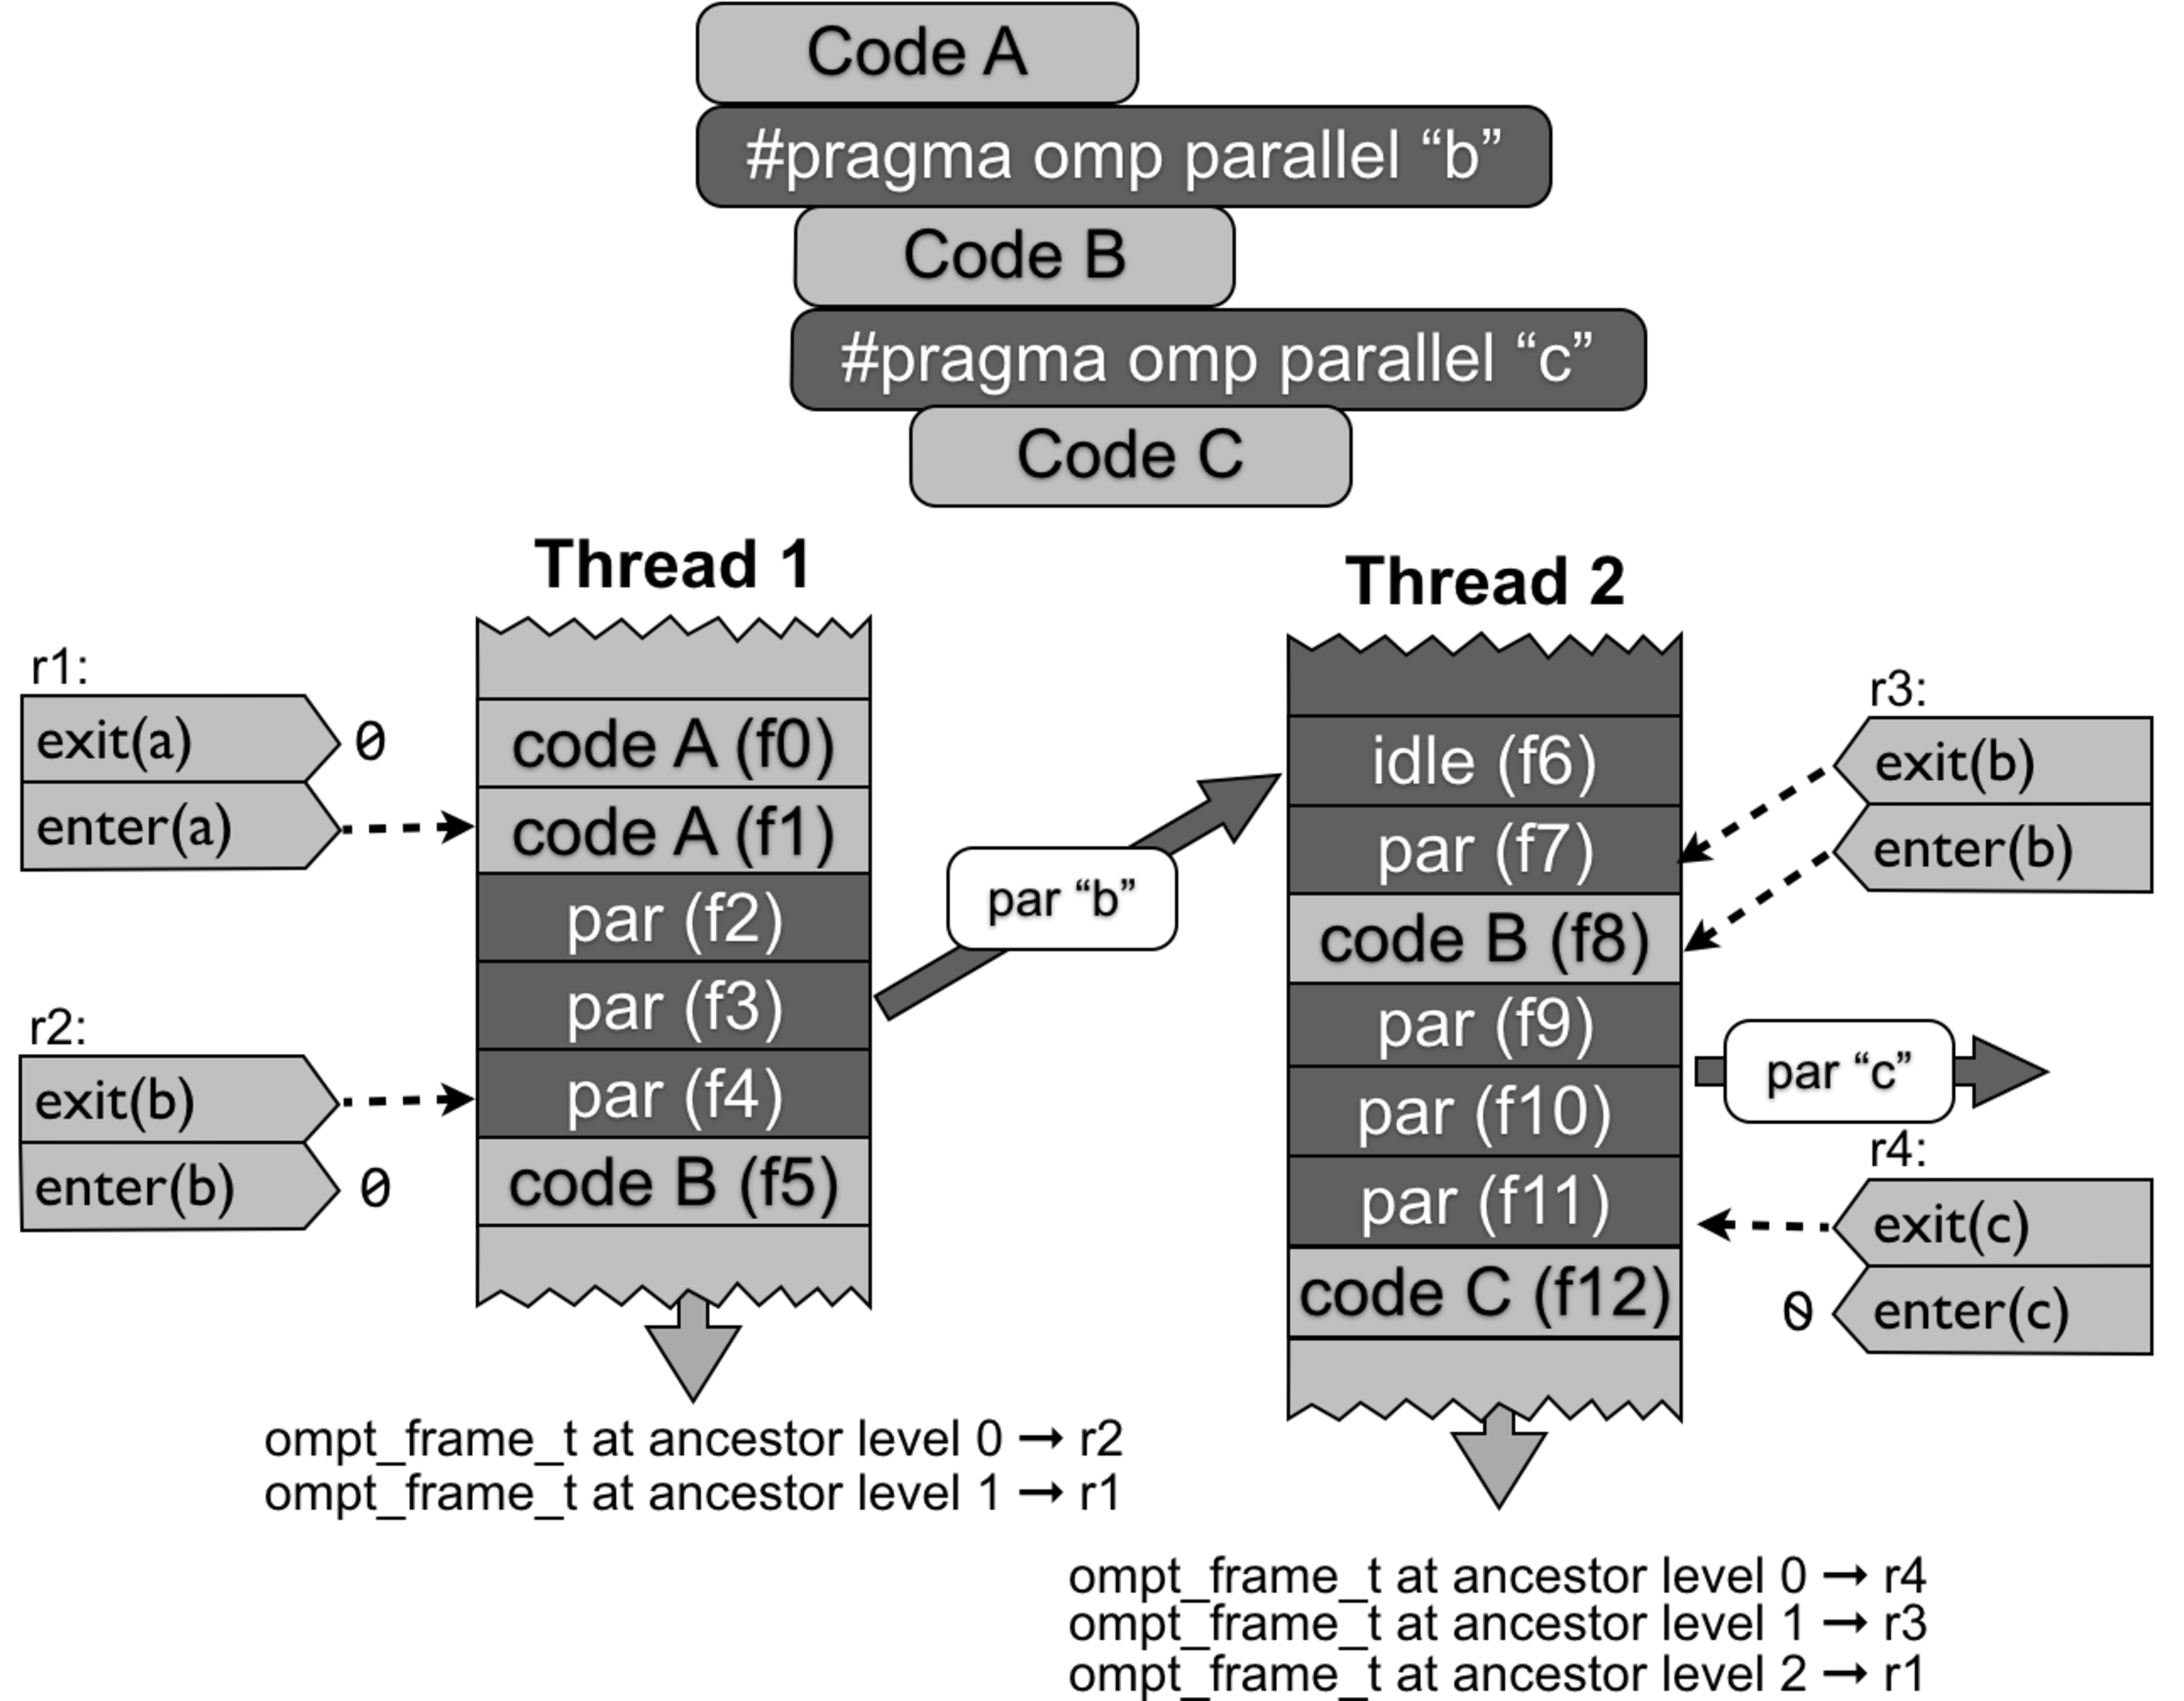
\includegraphics[scale=0.55]{callstack-cropped.pdf}
    \caption{Frame information.}
    \label{fig:frame}
\end{figure}

\noindent
Figure~\ref{fig:frame} illustrates a program executing a nested parallel region, where code A, B, and C represent, respectively, code associated with an initial task, outer-parallel, and inner-parallel regions.  Figure~\ref{fig:frame}  also depicts the stacks of two threads, where each new function call instantiates a new stack frame below the previous frames. When thread 1 encounters the outer-parallel region (parallel ``b"), it calls a routine in the OpenMP runtime system to create a new parallel region. The OpenMP runtime sets the \verb|reenter_runtime_frame| field in the \verb|ompt_frame_t| for the initial task executing code A to  frame f1---the user frame in the initial task that calls the runtime. The  \verb|ompt_frame_t| for the initial task is labeled  \verb|r1| in Figure~\ref{fig:frame}. In this figure, three consecutive runtime system frames (labeled ``par'' with frame identifiers f2--f4) are on the stack. 
Before starting the implicit task for parallel region ``b" in thread 1, the runtime sets the \verb|exit_runtime_frame| in the implicit task's \verb|ompt_frame_t|  (labeled \verb|r2|) to f4. Execution of application code for parallel region ``b''  begins on thread 1  when the runtime system invokes application code B (frame f5) from frame f4. 

Let us focus now on thread 2, an OpenMP thread. Figure~\ref{fig:frame}  shows this worker executing  work for the outer-parallel region ``b."
On the OpenMP thread's stack is a runtime frame labeled ``idle,'' where the OpenMP thread waits for work. 
When work becomes available, the runtime system invokes a function to dispatch it. While dispatching parallel work might involve a chain of several calls, here we assume that the length of this chain is 1 (frame f7).  Before thread 2 exits the runtime to execute an implicit task for parallel region ``b,'' the runtime 
sets the \verb|exit_runtime_frame| field of the implicit task's \verb|ompt_frame_t| (labeled \verb|r3|) to frame f7. 
When thread 2 later encounters the inner-parallel region ``c,"  as execution returns to the runtime,  the runtime fills in the  \verb|reenter_runtime_frame| field of the current task's \verb|ompt_frame_t| (labeled \verb|r3|) to frame f8---the frame that invoked the runtime. Before the task for parallel region ``c'' is invoked on thread 2, the runtime system sets the \verb|exit_runtime_frame| field  of the \verb|ompt_frame_t| (labeled \verb|r4|) for the implicit task for ``c'' 
to frame f11. Execution of application code for parallel region ``c''  begins on thread 2  when the runtime system invokes application code C (frame f12) from frame f11.


Below the stack for each thread in Figure~\ref{fig:frame}, the figure shows the \verb|ompt_frame_t| information obtained by calls to \verb|ompt_get_task_info| made on each thread for the stack state shown. We show the ID of the \verb|ompt_frame_t| record returned at each ancestor level. Note that thread 2 has task frame information for three levels of tasks, whereas thread 1 has only two.

\clearpage
\section{Implementation Considerations for Tool  Registration}
\label{app:registration} 

Whether a tool-supplied implementation of  \verb|ompt_tool| defined as a strong global symbol is visible to an OpenMP runtime system when present in the address space of a process is non-obvious. There are several scenarios to consider.
A tool-supplied version of \verb|ompt_tool|  is visible to an OpenMP runtime system if:
\begin{itemize}
\item The tool implementation of  \verb|ompt_tool| is statically-linked into an executable. Such an implementation of  \verb|ompt_tool| will  be visible to an OpenMP runtime system regardless of whether the runtime is statically linked into the executable or dynamically-linked into a shared library. 
\item An implementation of  \verb|ompt_tool|  is in a tool's shared library, which we denote ${\cal L}_T$. Such an implementation of  \verb|ompt_tool| will  be visible to an OpenMP runtime system in a library ${\cal L}_O$ as long as (a) ${\cal L}_O$ is a shared library itself, and (b) ${\cal L}_T$ is in the dynamic library search path for ${\cal L}_O$ ahead of ${\cal L}_O$  itself. ${\cal L}_T$ is guaranteed to be on ${\cal L}_O$'s dynamic library search path ahead of ${\cal L}_O$ {\em iff}
\begin{itemize}
\item ${\cal L}_T$ is pre-loaded by the dynamic linker into the address space of a process before execution begins.\footnote{While Linux and some other operating systems support library pre-loading, library pre-loading is not universally available.}
\item ${\cal L}_T$ and ${\cal L}_O$ are both direct shared library dependences of a load module\footnote{A load module is an application binary or a  shared library.}  and ${\cal L}_T$ appeared ahead of ${\cal L}_O$ when linking the load module.
\item A load module dynamically loads ${\cal L}_T$  ahead of a shared library ${\cal L}_X$ (because ${\cal L}_T$  preceded ${\cal L}_X$ when the load module was linked), and  ${\cal L}_X$ directly or indirectly loads ${\cal L}_O$.
\end{itemize}
\end{itemize}

The recommended approach for handling registration in the OpenMP runtime system for a particular target platform depends on the features supported by  compiler, linker, and operating system.

\paragraph{Compiler and linker support weak symbols.}
On systems  where the compiler and linker support weak symbols, it is convenient for the 
OpenMP runtime system to define \verb|ompt_tool| as a weak global symbol  that returns 0. Definition of \verb|ompt_tool| as a weak global symbol is suitable for use in either a static or dynamic library. If a shared-library implementation of an OpenMP library ${\cal L}_O$ defines \verb|ompt_tool| as a weak global symbol, then a tool library  ${\cal L}_T$ must be appear on the dynamic library search path ahead of ${\cal L}_O$ for the tool version of  \verb|ompt_tool| to be invoked.

\paragraph{Compiler and linker don't support weak symbols.}

On systems that don't support weak symbols, different implementation strategies are needed for static and dynamic linking. 

For a static library implementation of an  OpenMP runtime library,  the library can provide a stub version of \verb|ompt_tool|  in a separate object file. In this case, the linker will include the OpenMP library's stub implementation of  \verb|ompt_tool| only if no tool supplied version is already present when the OpenMP runtime library is used to resolve undefined symbols.

An OpenMP implementation used as a dynamic library can define \verb|ompt_tool| as a global symbol. The version in the OpenMP library would  be invoked only if no tool-supplied implementation of  \verb|ompt_tool| is statically linked in the executable or  a tool library that appears before the OpenMP runtime library in the dynamic library search path during execution.

\paragraph{A Binary rewriter alters a load module that provides an OpenMP runtime system.}
Regardless of whether a system supports weak symbols or not, one can use a static or dynamic binary rewriting tool to modify an 
OpenMP runtime system present in an executable or a shared library to invoke a tool-supplied version of 
a version of \verb|ompt_tool| rather than the default implementation of \verb|ompt_tool| present in the OpenMP runtime.



\end{document}
